\chapter{Denoobification: Maßtheorie}

Dieses Kapitel führt in die grundlegenden Konzepte der Maßtheorie ein, die für ein tiefes Verständnis der Stochastischen Calculus unerlässlich sind. Wenn Sie bereits mit diesen Konzepten vertraut sind, können Sie dieses Kapitel überspringen.

\section{Einleitung: Warum Maßtheorie?}

Die Maßtheorie ist das mathematische Fundament der modernen Wahrscheinlichkeitstheorie. Sie ermöglicht es uns:
\begin{itemize}
    \item Präzise zu definieren, was "Wahrscheinlichkeit" bedeutet
    \item Mit unendlichen Mengen und kontinuierlichen Verteilungen zu arbeiten
    \item Integrationstheorie rigoros zu entwickeln
    \item Stochastische Prozesse zu verstehen
\end{itemize}

\textbf{Intuition:} In der Schule lernt man Wahrscheinlichkeit oft als "Anzahl günstiger Fälle / Anzahl möglicher Fälle". Die Maßtheorie verallgemeinert dies auf unendliche Mengen und abstrakte Räume.

\section{\texorpdfstring{$\sigma$-Algebra}{sigma-Algebra}}

\begin{center}
\begin{tikzpicture}[scale=0.85]
    % Omega (Grundmenge)
    \node[ellipse, draw=blue!70!black, very thick, minimum width=5cm, minimum height=3.5cm, fill=blue!5] (omega) at (0,0) {};
    \node[above] at (omega.north) {\Large $\Omega$ (Grundmenge)};
    
    % Teilmengen in F
    \node[circle, draw=red!70!black, thick, minimum size=1.5cm, fill=red!20] (A1) at (-1.5, 0.5) {$A_1$};
    \node[circle, draw=red!70!black, thick, minimum size=1.2cm, fill=red!20] (A2) at (1, 0.8) {$A_2$};
    \node[circle, draw=red!70!black, thick, minimum size=1cm, fill=red!20] (A3) at (0, -1) {$A_3$};
    
    % Komplemente (gestrichelt)
    \draw[green!70!black, dashed, thick] (-2.5, -1.5) arc (180:360:2.5cm and 1.5cm);
    \node[above left] at (-2.3, 0.3) {\small $A_1^c$};
    
    % Vereinigung (gestrichelt)
    \draw[orange!70!black, dashed, thick] (-2, -1.2) rectangle (2, 1.5);
    \node[above] at (0, 1.3) {\small $\bigcup A_i$};
    
    % Label für sigma-Algebra
    \node[below] at (omega.south) {\textbf{$\sigma$-Algebra $\mathcal{F}$:} Enthält $\Omega$, Komplemente, Vereinigungen};
    
    % Legende
    \node[rectangle, draw=black, fill=white, text width=3cm] at (6, 1) {
        \small
        \textcolor{red!70!black}{$\bullet$} Mengen in $\mathcal{F}$ \\
        \textcolor{green!70!black}{$\bullet$} Komplemente \\
        \textcolor{orange!70!black}{$\bullet$} Vereinigungen
    };
\end{tikzpicture}
\end{center}

\begin{denoobification}[$\sigma$-Algebra]
\textbf{Was ist eine $\sigma$-Algebra?}

Eine \textbf{$\sigma$-Algebra} $\mathcal{F}$ auf einer Menge $\Omega$ ist eine Sammlung von Teilmengen von $\Omega$, die folgende Eigenschaften hat:

\begin{enumerate}
    \item \textbf{Enthält die Grundmenge:} $\Omega \in \mathcal{F}$
    \item \textbf{Abgeschlossen unter Komplement:} Wenn $A \in \mathcal{F}$, dann auch $A^c = \Omega \setminus A \in \mathcal{F}$
    \item \textbf{Abgeschlossen unter abzählbaren Vereinigungen:} Wenn $A_1, A_2, A_3, \ldots \in \mathcal{F}$, dann auch $\bigcup_{i=1}^{\infty} A_i \in \mathcal{F}$
\end{enumerate}

\textbf{Intuition:} Eine $\sigma$-Algebra beschreibt, welche Teilmengen von $\Omega$ wir "messen" können. Sie ist die mathematische Formalisierung von "messbaren Ereignissen".

\textbf{Beispiele:}
\begin{itemize}
    \item \textbf{Triviale $\sigma$-Algebra:} $\mathcal{F} = \{\emptyset, \Omega\}$ - die kleinste $\sigma$-Algebra
    \item \textbf{Diskrete $\sigma$-Algebra:} Für endliche $\Omega$ ist oft $\mathcal{F} = 2^{\Omega}$ (alle Teilmengen)
    \item \textbf{Borel-$\sigma$-Algebra:} Auf $\mathbb{R}$ ist $\mathcal{B}(\mathbb{R})$ die kleinste $\sigma$-Algebra, die alle offenen Intervalle enthält
\end{itemize}

\textbf{Warum wichtig?} In der Wahrscheinlichkeitstheorie beschreibt $\mathcal{F}$ alle "Ereignisse", denen wir eine Wahrscheinlichkeit zuordnen können.

\textbf{Industrielle Anwendung (Elektrotechnik/Informatik):}
\begin{itemize}
    \item \textbf{Digitale Signalverarbeitung:} In einem digitalen Filter beschreibt $\mathcal{F}$ alle möglichen Signalzustände, die gemessen werden können (z.B. Spannungswerte in bestimmten Bereichen)
    \item \textbf{Fehlererkennung:} In einem Kommunikationssystem beschreibt $\mathcal{F}$ alle möglichen Fehlerereignisse (Bitfehler, Paketverlust, etc.), denen Wahrscheinlichkeiten zugeordnet werden
    \item \textbf{Sensorik:} Bei einem Temperatursensor beschreibt $\mathcal{F}$ alle messbaren Temperaturbereiche - nur diese können als "Ereignisse" behandelt werden
\end{itemize}

\textbf{Mars-Kolonisierung Anwendung:}
\begin{itemize}
    \item \textbf{Lebenserhaltungssysteme:} $\mathcal{F}$ beschreibt alle messbaren Zustände des Lebenserhaltungssystems (Sauerstoffgehalt, Druck, Temperatur) - nur diese können überwacht und gesteuert werden
    \item \textbf{Ressourcen-Management:} Die $\sigma$-Algebra beschreibt alle messbaren Ressourcenzustände (Wasservorrat, Energie, Nahrung) - essentiell für die Überlebensplanung
    \item \textbf{Umwelt-Monitoring:} $\mathcal{F}$ beschreibt alle messbaren Mars-Umweltbedingungen (Strahlung, Staubstürme, Temperaturschwankungen), die das Überleben beeinflussen können
\end{itemize}

\textbf{$\star$ Mental Model zum Auswendiglernen:}
\begin{itemize}
    \item \textbf{Analogie:} Eine $\sigma$-Algebra ist wie ein "Messgerät" - sie sagt, welche Ereignisse wir überhaupt messen können
    \item \textbf{Merksatz:} "$\sigma$ = Sigma = Sammlung von messbaren Mengen"
    \item \textbf{3 Regeln:} (1) Enthält $\Omega$, (2) Abgeschlossen unter Komplement, (3) Abgeschlossen unter abzählbaren Vereinigungen
    \item \textbf{Visualisierung:} Stellen Sie sich $\Omega$ als eine große Box vor. Die $\sigma$-Algebra ist eine Sammlung von "Teilboxen", die wir öffnen und messen können
\end{itemize}
\end{denoobification}

\begin{denoobification}[Erzeugte $\sigma$-Algebra]
\textbf{Was ist eine erzeugte $\sigma$-Algebra?}

Sei $\mathcal{E}$ eine Sammlung von Teilmengen von $\Omega$. Die \textbf{von $\mathcal{E}$ erzeugte $\sigma$-Algebra} $\sigma(\mathcal{E})$ ist die kleinste $\sigma$-Algebra, die $\mathcal{E}$ enthält.

\textbf{Konstruktion:}
\begin{enumerate}
    \item Beginne mit $\mathcal{E}$
    \item Füge alle Komplemente hinzu
    \item Füge alle abzählbaren Vereinigungen hinzu
    \item Wiederhole, bis keine neuen Mengen mehr hinzukommen
\end{enumerate}

\textbf{Beispiele:}
\begin{itemize}
    \item $\sigma(\{(1,2)\}) = \{\emptyset, (1,2), (1,2)^c, \mathbb{R}\}$ auf $\mathbb{R}$
    \item $\sigma(\text{offene Intervalle}) = \mathcal{B}(\mathbb{R})$ (Borel-$\sigma$-Algebra)
    \item In der Wahrscheinlichkeit: $\sigma(X)$ ist die $\sigma$-Algebra, die von der Zufallsvariable $X$ erzeugt wird
\end{itemize}

\textbf{Intuition:} Die erzeugte $\sigma$-Algebra ist die "minimale" $\sigma$-Algebra, die alle Mengen aus $\mathcal{E}$ enthält.

\textbf{Industrielle Anwendung (Elektrotechnik/Informatik):}
\begin{itemize}
    \item \textbf{Sensor-Fusion:} Wenn mehrere Sensoren (Temperatur, Druck, Beschleunigung) Messwerte liefern, erzeugt die Menge aller möglichen Sensor-Kombinationen eine $\sigma$-Algebra für die gemeinsame Auswertung
    \item \textbf{AD-Wandler:} Die von den Quantisierungsstufen erzeugte $\sigma$-Algebra beschreibt alle messbaren Spannungsbereiche in einem Analog-Digital-Wandler
    \item \textbf{Netzwerk-Monitoring:} Die von Basis-Ereignissen (Paketankunft, Verbindungsaufbau) erzeugte $\sigma$-Algebra beschreibt alle analysierbaren Netzwerkereignisse
\end{itemize}

\textbf{Mars-Kolonisierung Anwendung:}
\begin{itemize}
    \item \textbf{Habitat-Sensor-Netzwerk:} Die von Basis-Sensoren (CO$_2$, O$_2$, Druck, Temperatur) erzeugte $\sigma$-Algebra beschreibt alle analysierbaren Habitat-Zustände - kritisch für automatische Lebenserhaltungssysteme
    \item \textbf{Rover-Navigation:} Die von Basis-Ereignissen (Fels, Sand, Krater) erzeugte $\sigma$-Algebra beschreibt alle navigierbaren Geländetypen auf dem Mars
    \item \textbf{Ressourcen-Erkundung:} Die von Basis-Fundstellen (Wassereis, Mineralien) erzeugte $\sigma$-Algebra beschreibt alle möglichen Ressourcen-Kombinationen, die gefunden werden können
\end{itemize}

\textbf{$\star$ Mental Model zum Auswendiglernen:}
\begin{itemize}
    \item \textbf{Analogie:} Wie ein "Hüllen-Operator" - nimmt eine Sammlung und macht sie zu einer vollständigen $\sigma$-Algebra
    \item \textbf{Merksatz:} "$\sigma(\mathcal{E})$ = kleinste $\sigma$-Algebra, die $\mathcal{E}$ enthält"
    \item \textbf{Prozess:} Starte mit $\mathcal{E}$ → füge Komplemente hinzu → füge Vereinigungen hinzu → wiederhole bis fertig
    \item \textbf{Visualisierung:} Wie eine "Schale", die um die ursprünglichen Mengen gebaut wird
\end{itemize}

\begin{center}
\begin{tikzpicture}[scale=0.9]
    % Omega
    \node[ellipse, draw=blue!70!black, thick, minimum width=4cm, minimum height=2.5cm, fill=blue!5] (omega) at (0,0) {};
    \node[above] at (omega.north) {$\Omega$};
    
    % Ursprüngliche Mengen E
    \node[circle, draw=red!70!black, thick, minimum size=0.8cm, fill=red!20] (E1) at (-1, 0.3) {$E_1$};
    \node[circle, draw=red!70!black, thick, minimum size=0.8cm, fill=red!20] (E2) at (1, 0.5) {$E_2$};
    \node[circle, draw=red!70!black, thick, minimum size=0.8cm, fill=red!20] (E3) at (0, -0.5) {$E_3$};
    
    % Erzeugte sigma-Algebra (größere Schale)
    \draw[green!70!black, dashed, very thick] (-2.5, -1.5) ellipse (2.5cm and 1.5cm);
    \node[above right] at (-2.3, 0.5) {\small $\sigma(\mathcal{E})$};
    
    % Pfeile zeigen Erweiterung
    \draw[->, thick, orange!70!black] (E1) to[bend left=20] node[above, sloped, font=\small] {Komplemente} (-1.5, 1);
    \draw[->, thick, orange!70!black] (E2) to[bend right=20] node[below, sloped, font=\small] {Vereinigungen} (1.5, -1);
    
    % Label
    \node[below] at (0, -2) {\textbf{Erzeugte $\sigma$-Algebra: Hülle um $\mathcal{E}$}};
    \node[above left] at (-3, 1.5) {\small \textcolor{red!70!black}{$\mathcal{E}$} (ursprünglich)};
    \node[above right] at (2, 1.5) {\small \textcolor{green!70!black}{$\sigma(\mathcal{E})$} (erzeugt)};
\end{tikzpicture}
\end{center}
\end{denoobification}

\section{Maß}

\begin{denoobification}[Maß]
\textbf{Was ist ein Maß?}

Ein \textbf{Maß} $\mu$ auf einem messbaren Raum $(\Omega, \mathcal{F})$ ist eine Funktion $\mu: \mathcal{F} \to [0, \infty]$, die folgende Eigenschaften hat:

\begin{enumerate}
    \item \textbf{Nicht-Negativität:} $\mu(A) \geq 0$ für alle $A \in \mathcal{F}$
    \item \textbf{Leere Menge:} $\mu(\emptyset) = 0$
    \item \textbf{$\sigma$-Additivität:} Für paarweise disjunkte Mengen $A_1, A_2, \ldots \in \mathcal{F}$ gilt:
    \[
    \mu\left(\bigcup_{i=1}^{\infty} A_i\right) = \sum_{i=1}^{\infty} \mu(A_i)
    \]
\end{enumerate}

\textbf{Intuition:} Ein Maß ordnet jeder messbaren Menge eine "Größe" zu. In der Wahrscheinlichkeit ist dies die "Wahrscheinlichkeit".

\textbf{Industrielle Anwendung (Elektrotechnik/Informatik):}
\begin{itemize}
    \item \textbf{Signalenergie:} In der Signalverarbeitung misst das Lebesgue-Maß die "Energie" eines Signals über einem Zeitintervall: $E = \int_{[t_1,t_2]} |s(t)|^2 dt$
    \item \textbf{Leistungsmessung:} In der Elektrotechnik misst ein Maß die durchschnittliche Leistung über einem Frequenzband: $P = \int_B S(f) df$, wobei $S(f)$ das Leistungsspektrum ist
    \item \textbf{Speicherplatz:} In der Informatik kann ein Maß die "Größe" von Datenmengen beschreiben (z.B. Anzahl Bytes in bestimmten Bereichen)
\end{itemize}

\textbf{Mars-Kolonisierung Anwendung:}
\begin{itemize}
    \item \textbf{Energie-Management:} Ein Maß beschreibt die verfügbare Solarenergie über einen Zeitraum: $E = \int_{[t_1,t_2]} P_{\text{solar}}(t) dt$ - kritisch für die Planung von Aktivitäten während der Marstage
    \item \textbf{Wasservorrat:} Ein Maß beschreibt die "Größe" des Wasservorrats in verschiedenen Speichern - essentiell für Überlebensplanung
    \item \textbf{Strahlungsdosis:} Ein Maß beschreibt die kumulative Strahlungsdosis über einen Zeitraum: $D = \int_{[0,t]} R(\tau) d\tau$ - wichtig für die Gesundheit der Kolonisten
    \item \textbf{Atmosphärendruck:} Ein Maß beschreibt die "Größe" des Druckbereichs im Habitat - muss innerhalb sicherer Grenzen bleiben
\end{itemize}

\textbf{Beispiele:}
\begin{itemize}
    \item \textbf{Zählmaß:} $\mu(A) =$ Anzahl der Elemente in $A$ (für endliche Mengen)
    \item \textbf{Lebesgue-Maß:} $\mu([a,b]) = b-a$ (Länge eines Intervalls)
    \item \textbf{Wahrscheinlichkeitsmaß:} $\mathbb{P}(\Omega) = 1$ (normiertes Maß)
\end{itemize}

\textbf{Eigenschaften:}
\begin{itemize}
    \item \textbf{Monotonie:} Wenn $A \subset B$, dann $\mu(A) \leq \mu(B)$
    \item \textbf{Subadditivität:} $\mu\left(\bigcup_{i=1}^{\infty} A_i\right) \leq \sum_{i=1}^{\infty} \mu(A_i)$
    \item \textbf{Stetigkeit von unten:} Wenn $A_1 \subset A_2 \subset \cdots$, dann $\mu\left(\bigcup_{i=1}^{\infty} A_i\right) = \lim_{i \to \infty} \mu(A_i)$
\end{itemize}

\textbf{$\star$ Mental Model zum Auswendiglernen:}
\begin{itemize}
    \item \textbf{Analogie:} Ein Maß ist wie eine "Waage" oder "Lineal" - es misst die "Größe" von Mengen
    \item \textbf{Merksatz:} "Maß = Funktion, die Mengen Zahlen zuordnet (ihre Größe)"
    \item \textbf{3 Eigenschaften:} (1) Nicht-negativ, (2) Leere Menge = 0, (3) $\sigma$-Additivität (Größe von Vereinigung = Summe der Größen)
    \item \textbf{Visualisierung:} Stellen Sie sich vor, Sie "wiegen" jede messbare Menge. Die Summe der Gewichte disjunkter Mengen ist das Gewicht ihrer Vereinigung
\end{itemize}

\begin{center}
\begin{tikzpicture}[scale=0.9]
    % Omega
    \node[ellipse, draw=blue!70!black, thick, minimum width=5cm, minimum height=3cm, fill=blue!5] (omega) at (0,0) {};
    \node[above] at (omega.north) {$\Omega$};
    
    % Disjunkte Mengen
    \node[circle, draw=red!70!black, thick, minimum size=1cm, fill=red!20] (A1) at (-1.5, 0.5) {$A_1$};
    \node[circle, draw=red!70!black, thick, minimum size=1.2cm, fill=red!20] (A2) at (0.5, 0.8) {$A_2$};
    \node[circle, draw=red!70!black, thick, minimum size=0.9cm, fill=red!20] (A3) at (1.5, -0.5) {$A_3$};
    
    % Maß-Werte
    \node[above] at (A1.north) {\small $\mu(A_1) = 2$};
    \node[above] at (A2.north) {\small $\mu(A_2) = 3$};
    \node[below] at (A3.south) {\small $\mu(A_3) = 1$};
    
    % Vereinigung
    \draw[green!70!black, dashed, very thick] (-2.5, -1.5) ellipse (2.5cm and 1.5cm);
    \node[above] at (0, 1.5) {\small $\bigcup A_i$};
    
    % sigma-Additivität
    \node[below] at (0, -2) {\small $\mu\left(\bigcup A_i\right) = \mu(A_1) + \mu(A_2) + \mu(A_3) = 2 + 3 + 1 = 6$};
    
    % Waage-Symbol
    \node[rectangle, draw=orange!70!black, thick, minimum width=1.5cm, minimum height=0.5cm, fill=orange!10] (scale) at (4, 0) {Waage};
    \draw[->, thick, orange!70!black] (A1) to[bend left=30] (scale);
    \draw[->, thick, orange!70!black] (A2) to (scale);
    \draw[->, thick, orange!70!black] (A3) to[bend right=30] (scale);
    
    % Label
    \node[below] at (0, -2.8) {\textbf{Maß: $\sigma$-Additivität für disjunkte Mengen}};
\end{tikzpicture}
\end{center}
\end{denoobification}

\begin{denoobification}[Wahrscheinlichkeitsmaß]
\textbf{Was ist ein Wahrscheinlichkeitsmaß?}

Ein \textbf{Wahrscheinlichkeitsmaß} $\mathbb{P}$ ist ein Maß mit $\mathbb{P}(\Omega) = 1$.

\textbf{Intuition:} Ein Wahrscheinlichkeitsmaß ordnet jedem Ereignis eine Wahrscheinlichkeit zwischen 0 und 1 zu, wobei das sichere Ereignis $\Omega$ die Wahrscheinlichkeit 1 hat.

\textbf{Beispiele:}
\begin{itemize}
    \item \textbf{Gleichverteilung auf endlicher Menge:} $\mathbb{P}(\{i\}) = \frac{1}{n}$ für $i = 1, \ldots, n$
    \item \textbf{Gleichverteilung auf $[0,1]$:} $\mathbb{P}([a,b]) = b-a$ für $0 \leq a \leq b \leq 1$
    \item \textbf{Normalverteilung:} $\mathbb{P}((-\infty, x]) = \Phi(x)$ (Verteilungsfunktion)
\end{itemize}

\textbf{Wahrscheinlichkeitsraum:} Ein Tripel $(\Omega, \mathcal{F}, \mathbb{P})$ heißt \textbf{Wahrscheinlichkeitsraum}.

\textbf{Industrielle Anwendung (Elektrotechnik/Informatik):}
\begin{itemize}
    \item \textbf{Zuverlässigkeitsanalyse:} In der Elektronik beschreibt $\mathbb{P}$ die Wahrscheinlichkeit, dass ein Bauteil innerhalb eines Zeitintervalls ausfällt: $\mathbb{P}(\text{Ausfall in } [0,t]) = 1 - e^{-\lambda t}$
    \item \textbf{Bitfehlerrate (BER):} In der Kommunikationstechnik ist $\mathbb{P}(\text{Bitfehler}) = p$ die Wahrscheinlichkeit eines Übertragungsfehlers
    \item \textbf{Qualitätskontrolle:} In der Produktion beschreibt $\mathbb{P}$ die Wahrscheinlichkeit, dass ein Produkt bestimmte Toleranzen erfüllt
    \item \textbf{Netzwerk-Performance:} $\mathbb{P}(\text{Paketverzögerung} > t)$ beschreibt die Wahrscheinlichkeit von Latenzproblemen
\end{itemize}

\textbf{Mars-Kolonisierung Anwendung:}
\begin{itemize}
    \item \textbf{Überlebenswahrscheinlichkeit:} $\mathbb{P}(\text{Überleben für } t \text{ Jahre})$ beschreibt die Wahrscheinlichkeit, dass ein Kolonist $t$ Jahre auf dem Mars überlebt - kritisch für Missionsplanung
    \item \textbf{System-Ausfall:} $\mathbb{P}(\text{Lebenserhaltungssystem fällt aus in } [0,t])$ beschreibt die Wahrscheinlichkeit eines kritischen Systemausfalls - bestimmt Redundanz-Anforderungen
    \item \textbf{Erfolgreiche Landung:} $\mathbb{P}(\text{Erfolgreiche Landung})$ beschreibt die Wahrscheinlichkeit einer sicheren Landung auf dem Mars - historisch etwa 50\%
    \item \textbf{Ressourcen-Verfügbarkeit:} $\mathbb{P}(\text{Wassereis gefunden in Region } A)$ beschreibt die Wahrscheinlichkeit, Ressourcen an einem bestimmten Ort zu finden
    \item \textbf{Erd-Kommunikation:} $\mathbb{P}(\text{Kommunikationsverlust} > t)$ beschreibt die Wahrscheinlichkeit, dass die Verbindung zur Erde für mehr als $t$ Stunden unterbrochen ist
\end{itemize}

\textbf{$\star$ Mental Model zum Auswendiglernen:}
\begin{itemize}
    \item \textbf{Analogie:} Ein Wahrscheinlichkeitsraum ist wie ein "Glücksspiel" - $\Omega$ = alle möglichen Ergebnisse, $\mathcal{F}$ = alle Ereignisse, $\mathbb{P}$ = Wahrscheinlichkeiten
    \item \textbf{Merksatz:} "Wahrscheinlichkeitsraum = (Ergebnisse, Ereignisse, Wahrscheinlichkeiten)"
    \item \textbf{3 Komponenten:} $\Omega$ (was passieren kann), $\mathcal{F}$ (was wir fragen können), $\mathbb{P}$ (wie wahrscheinlich)
    \item \textbf{Visualisierung:} Wie ein Würfel: $\Omega = \{1,2,3,4,5,6\}$, $\mathcal{F}$ = alle Teilmengen, $\mathbb{P}(\{i\}) = 1/6$
\end{itemize}

\begin{center}
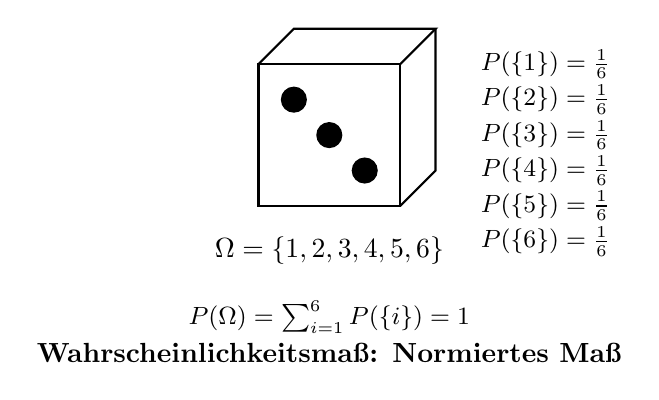
\begin{tikzpicture}[scale=0.9]
    % Würfel-Darstellung
    \draw[thick] (0,0) rectangle (2,2);
    \draw[thick] (0,2) -- (0.5,2.5) -- (2.5,2.5) -- (2,2);
    \draw[thick] (2,0) -- (2.5,0.5) -- (2.5,2.5);
    
    % Würfelpunkte
    \node[circle, fill=black] at (0.5, 1.5) {};
    \node[circle, fill=black] at (1.5, 0.5) {};
    \node[circle, fill=black] at (1, 1) {};
    
    % Omega
    \node[below] at (1, -0.3) {$\Omega = \{1,2,3,4,5,6\}$};
    
    % Wahrscheinlichkeiten
    \node[right] at (3, 2) {\small $\mathbb{P}(\{1\}) = \frac{1}{6}$};
    \node[right] at (3, 1.5) {\small $\mathbb{P}(\{2\}) = \frac{1}{6}$};
    \node[right] at (3, 1) {\small $\mathbb{P}(\{3\}) = \frac{1}{6}$};
    \node[right] at (3, 0.5) {\small $\mathbb{P}(\{4\}) = \frac{1}{6}$};
    \node[right] at (3, 0) {\small $\mathbb{P}(\{5\}) = \frac{1}{6}$};
    \node[right] at (3, -0.5) {\small $\mathbb{P}(\{6\}) = \frac{1}{6}$};
    
    % Normierung
    \node[below] at (1, -1.2) {\small $\mathbb{P}(\Omega) = \sum_{i=1}^{6} \mathbb{P}(\{i\}) = 1$};
    
    % Label
    \node[below] at (1, -1.8) {\textbf{Wahrscheinlichkeitsmaß: Normiertes Maß}};
\end{tikzpicture}
\end{center}
\end{denoobification}

\section{Messbare Funktionen}

\begin{denoobification}[Messbare Funktion]
\textbf{Was ist eine messbare Funktion?}

Eine Funktion $f: (\Omega, \mathcal{F}) \to (\mathbb{R}, \mathcal{B}(\mathbb{R}))$ heißt \textbf{messbar}, wenn für jedes Borel-Menge $B \in \mathcal{B}(\mathbb{R})$ gilt:
\[
f^{-1}(B) = \{\omega \in \Omega : f(\omega) \in B\} \in \mathcal{F}
\]

\textbf{Intuition:} Eine messbare Funktion ist eine Funktion, bei der das Urbild jeder messbaren Menge wieder messbar ist.

\textbf{Äquivalente Definitionen:}
\begin{itemize}
    \item $f^{-1}((-\infty, a]) \in \mathcal{F}$ für alle $a \in \mathbb{R}$
    \item $f^{-1}((a, \infty)) \in \mathcal{F}$ für alle $a \in \mathbb{R}$
    \item $f^{-1}((a, b)) \in \mathcal{F}$ für alle $a < b$
\end{itemize}

\textbf{Beispiele:}
\begin{itemize}
    \item Jede stetige Funktion ist messbar (bezüglich Borel-$\sigma$-Algebra)
    \item Jede monotone Funktion ist messbar
    \item Zufallsvariablen sind messbare Funktionen!
\end{itemize}

\textbf{Warum wichtig?} Nur für messbare Funktionen können wir Integrale definieren.

\textbf{Industrielle Anwendung (Elektrotechnik/Informatik):}
\begin{itemize}
    \item \textbf{Analog-Digital-Wandler (ADC):} Die Umwandlung eines analogen Signals $s(t)$ in digitale Werte ist eine messbare Funktion - jeder Spannungsbereich wird auf einen diskreten Wert abgebildet
    \item \textbf{Signalverarbeitung:} Filterfunktionen $H(f)$ (Frequenzgang) sind messbar - sie ordnen Frequenzen messbare Amplituden zu
    \item \textbf{Sensor-Kalibrierung:} Die Kalibrierungsfunktion eines Sensors $f: \text{Physikalische Größe} \to \text{Spannung}$ muss messbar sein, um statistisch analysierbar zu sein
    \item \textbf{Feature-Extraktion:} In der Mustererkennung sind Extraktionsfunktionen (z.B. FFT-Koeffizienten) messbare Abbildungen von Signalen auf Feature-Vektoren
\end{itemize}

\textbf{Mars-Kolonisierung Anwendung:}
\begin{itemize}
    \item \textbf{Atmosphären-Analyse:} Die Funktion $f: \text{Mars-Atmosphäre} \to \text{CO}_2\text{-Konzentration}$ ist messbar - jeder Atmosphärenzustand wird auf eine messbare Konzentration abgebildet
    \item \textbf{Boden-Analyse:} Die Funktion $f: \text{Bodenprobe} \to \text{Mineralien-Konzentration}$ ist messbar - wichtig für Ressourcen-Erkundung
    \item \textbf{Strahlungs-Monitoring:} Die Funktion $f: \text{Umgebung} \to \text{Strahlungsdosis}$ ist messbar - kritisch für die Sicherheit der Kolonisten
    \item \textbf{Rover-Navigation:} Die Funktion $f: \text{Gelände} \to \text{Fahrbarkeit}$ ist messbar - jeder Geländetyp wird auf einen Fahrbarkeitswert abgebildet
\end{itemize}

\textbf{$\star$ Mental Model zum Auswendiglernen:}
\begin{itemize}
    \item \textbf{Analogie:} Eine messbare Funktion ist wie ein "Übersetzer" - übersetzt Ergebnisse in Zahlen, aber nur auf eine "messbare" Weise
    \item \textbf{Merksatz:} "Messbar = Urbild jeder messbaren Menge ist wieder messbar"
    \item \textbf{Test:} Wenn $f^{-1}((-\infty, a]) \in \mathcal{F}$ für alle $a$, dann ist $f$ messbar
    \item \textbf{Visualisierung:} Stellen Sie sich vor: Jede "Zahl-Box" auf der reellen Achse hat ein "Urbild" in $\Omega$, das messbar sein muss
\end{itemize}

\begin{center}
\begin{tikzpicture}[scale=0.9]
    % Omega
    \node[ellipse, draw=blue!70!black, thick, minimum width=3cm, minimum height=2cm, fill=blue!5] (omega) at (0,0) {$\Omega$};
    
    % Funktion f
    \draw[->, thick, red!70!black] (omega) to[bend left=30] node[above, sloped] {$f$} (4,0);
    
    % Reelle Achse
    \draw[->, thick] (4,0) -- (8,0) node[right] {$\mathbb{R}$};
    
    % Borel-Menge B
    \draw[green!70!black, very thick] (5, -0.3) -- (7, -0.3) -- (7, 0.3) -- (5, 0.3) -- cycle;
    \node[above] at (6, 0.3) {$B \in \mathcal{B}(\mathbb{R})$};
    
    % Urbild f^{-1}(B)
    \draw[orange!70!black, dashed, very thick] (-1.5, -1) ellipse (1.5cm and 1cm);
    \node[below] at (-1.5, -1) {$f^{-1}(B)$};
    
    % Pfeil zeigt Urbild
    \draw[->, thick, orange!70!black] (6, -0.3) to[bend right=40] node[below, sloped] {$f^{-1}$} (-1.5, -0.5);
    
    % Messbarkeits-Bedingung
    \node[below] at (0, -2.2) {\small $f$ messbar $\Leftrightarrow$ $f^{-1}(B) \in \mathcal{F}$ für alle $B \in \mathcal{B}(\mathbb{R})$};
    
    % Label
    \node[below] at (4, -2.8) {\textbf{Messbare Funktion: Urbild jeder Borel-Menge ist messbar}};
\end{tikzpicture}
\end{center}
\end{denoobification}

\begin{denoobification}[Einfache Funktion]
\textbf{Was ist eine einfache Funktion?}

Eine \textbf{einfache Funktion} ist eine Funktion der Form:
\[
f(\omega) = \sum_{i=1}^{n} a_i \mathbf{1}_{A_i}(\omega)
\]
wobei $a_i \in \mathbb{R}$ und $A_i \in \mathcal{F}$ disjunkte Mengen sind.

\textbf{Intuition:} Eine einfache Funktion nimmt nur endlich viele Werte an.

\textbf{Beispiele:}
\begin{itemize}
    \item Indikatorfunktion: $\mathbf{1}_A(\omega) = 1$ wenn $\omega \in A$, sonst $0$
    \item Treppenfunktion: $f(x) = 1$ für $x \in [0,1)$, $f(x) = 2$ für $x \in [1,2)$, etc.
\end{itemize}

\textbf{Approximationssatz:} Jede nicht-negative messbare Funktion kann durch einfache Funktionen approximiert werden:
\[
f_n(\omega) = \sum_{k=0}^{n2^n - 1} \frac{k}{2^n} \mathbf{1}_{\{k/2^n \leq f < (k+1)/2^n\}}(\omega) + n \mathbf{1}_{\{f \geq n\}}(\omega)
\]

\textbf{Industrielle Anwendung (Elektrotechnik/Informatik):}
\begin{itemize}
    \item \textbf{Quantisierung:} In der Digitalisierung wird ein kontinuierliches Signal durch eine einfache Funktion approximiert - jeder Quantisierungsschritt entspricht einem Wert $a_i$ auf einem Intervall
    \item \textbf{PWM (Pulsweitenmodulation):} Die Erzeugung von PWM-Signalen verwendet einfache Funktionen - konstante Werte über Zeitintervallen
    \item \textbf{Digital-Analog-Wandler (DAC):} Die Rekonstruktion eines Signals aus digitalen Werten ist eine einfache Funktion - Treppenfunktion mit endlich vielen Stufen
    \item \textbf{Histogramm-Berechnung:} In der Bildverarbeitung werden Pixelwerte in Bins gruppiert - dies entspricht einer einfachen Funktion
\end{itemize}

\textbf{Mars-Kolonisierung Anwendung:}
\begin{itemize}
    \item \textbf{Temperatur-Regelung:} Die Heizung/Kühlung im Habitat verwendet einfache Funktionen - konstante Werte über Zeitintervallen (z.B. Tag/Nacht-Zyklen)
    \item \textbf{Ressourcen-Alarmierung:} Die Warnfunktion für Ressourcen verwendet einfache Funktionen - diskrete Warnstufen (niedrig, kritisch, leer)
    \item \textbf{Energie-Management:} Die Energieverteilung verwendet einfache Funktionen - diskrete Prioritätsstufen für verschiedene Systeme
    \item \textbf{Rover-Steuerung:} Die Geschwindigkeitssteuerung eines Rovers verwendet einfache Funktionen - diskrete Geschwindigkeitsstufen je nach Geländetyp
\end{itemize}

\begin{center}
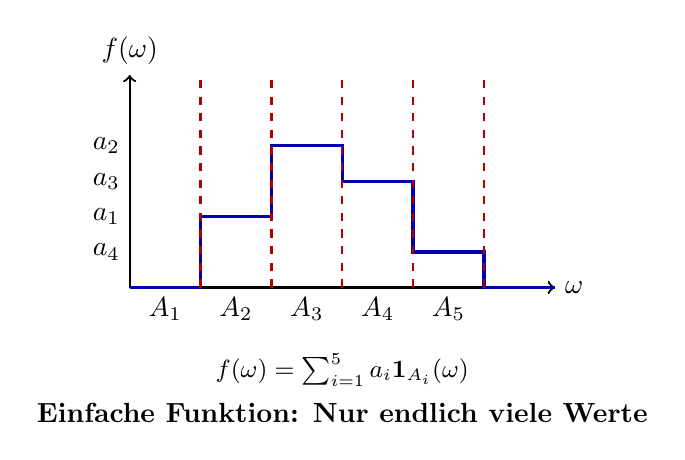
\begin{tikzpicture}[scale=0.9]
    % x-Achse
    \draw[->, thick] (0,0) -- (6,0) node[right] {$\omega$};
    \draw[->, thick] (0,0) -- (0,3) node[above] {$f(\omega)$};
    
    % Treppenfunktion (einfache Funktion)
    \draw[blue!70!black, very thick] (0,0) -- (1,0) -- (1,1) -- (2,1) -- (2,2) -- (3,2) -- (3,1.5) -- (4,1.5) -- (4,0.5) -- (5,0.5) -- (5,0) -- (6,0);
    
    % Werte markieren
    \node[left] at (0,1) {$a_1$};
    \node[left] at (0,2) {$a_2$};
    \node[left] at (0,1.5) {$a_3$};
    \node[left] at (0,0.5) {$a_4$};
    
    % Mengen markieren
    \draw[red!70!black, dashed, thick] (1,0) -- (1,3);
    \draw[red!70!black, dashed, thick] (2,0) -- (2,3);
    \draw[red!70!black, dashed, thick] (3,0) -- (3,3);
    \draw[red!70!black, dashed, thick] (4,0) -- (4,3);
    \draw[red!70!black, dashed, thick] (5,0) -- (5,3);
    
    \node[below] at (0.5, 0) {$A_1$};
    \node[below] at (1.5, 0) {$A_2$};
    \node[below] at (2.5, 0) {$A_3$};
    \node[below] at (3.5, 0) {$A_4$};
    \node[below] at (4.5, 0) {$A_5$};
    
    % Formel
    \node[below] at (3, -0.8) {\small $f(\omega) = \sum_{i=1}^{5} a_i \mathbf{1}_{A_i}(\omega)$};
    
    % Label
    \node[below] at (3, -1.5) {\textbf{Einfache Funktion: Nur endlich viele Werte}};
\end{tikzpicture}
\end{center}
\end{denoobification}

\section{Integration}

\begin{denoobification}[Lebesgue-Integral]
\textbf{Was ist das Lebesgue-Integral?}

Das \textbf{Lebesgue-Integral} ist eine Verallgemeinerung des Riemann-Integrals, die für messbare Funktionen auf messbaren Räumen definiert ist.

\textbf{Konstruktion (für nicht-negative Funktionen):}
\begin{enumerate}
    \item \textbf{Einfache Funktionen:} Für $f = \sum_{i=1}^{n} a_i \mathbf{1}_{A_i}$ definiere:
    \[
    \int f \, d\mu = \sum_{i=1}^{n} a_i \mu(A_i)
    \]
    \item \textbf{Allgemeine Funktionen:} Für messbare $f \geq 0$:
    \[
    \int f \, d\mu = \sup\left\{\int g \, d\mu : g \text{ einfach}, 0 \leq g \leq f\right\}
    \]
    \item \textbf{Allgemeine Funktionen:} Für beliebige $f$ schreibe $f = f^+ - f^-$ mit $f^+ = \max(f, 0)$ und $f^- = \max(-f, 0)$, dann:
    \[
    \int f \, d\mu = \int f^+ \, d\mu - \int f^- \, d\mu
    \]
    (falls nicht beide Integrale $\infty$ sind)
\end{enumerate}

\textbf{Intuition:} Das Lebesgue-Integral "misst" die Fläche unter der Funktion, aber nicht durch Rechtecke (wie Riemann), sondern durch messbare Mengen.

\textbf{Vorteile gegenüber Riemann:}
\begin{itemize}
    \item Funktioniert für mehr Funktionen
    \item Bessere Konvergenzsätze (Satz von Lebesgue)
    \item Natürlich für Wahrscheinlichkeitstheorie
\end{itemize}

\textbf{In der Wahrscheinlichkeit:} $\int X \, d\mathbb{P} = \mathbb{E}[X]$ (Erwartungswert!)

\textbf{Industrielle Anwendung (Elektrotechnik/Informatik):}
\begin{itemize}
    \item \textbf{Effektivwert (RMS):} Der Effektivwert eines Wechselstroms ist ein Lebesgue-Integral: $U_{\text{RMS}} = \sqrt{\frac{1}{T}\int_0^T u(t)^2 dt}$
    \item \textbf{Signalenergie:} Die Gesamtenergie eines Signals: $E = \int_{-\infty}^{\infty} |s(t)|^2 dt$ (Parseval-Theorem)
    \item \textbf{Leistungsspektrum:} Die durchschnittliche Leistung über einem Frequenzband: $P = \int_{f_1}^{f_2} S(f) df$, wobei $S(f)$ das Leistungsspektrum ist
    \item \textbf{Erwartungswert von Rauschen:} $\mathbb{E}[N(t)] = \int n \cdot f_N(n) dn$ beschreibt den Mittelwert von Rauschen in einem System
    \item \textbf{Filter-Response:} Die Ausgangsleistung eines Filters: $P_{\text{out}} = \int |H(f)|^2 S_{\text{in}}(f) df$
\end{itemize}

\textbf{Mars-Kolonisierung Anwendung:}
\begin{itemize}
    \item \textbf{Energieverbrauch:} Die Gesamtenergie über einen Marstag: $E = \int_{0}^{T_{\text{Tag}}} P(t) dt$ - kritisch für Solarenergie-Planung
    \item \textbf{Sauerstoff-Produktion:} Die kumulative Sauerstoffproduktion: $O_2 = \int_{0}^{t} r(\tau) d\tau$, wobei $r(t)$ die Produktionsrate ist
    \item \textbf{Wasserverbrauch:} Die Gesamtwassermenge über einen Zeitraum: $W = \int_{t_1}^{t_2} w(t) dt$ - essentiell für Überlebensplanung
    \item \textbf{Strahlungsdosis:} Die kumulative Strahlungsdosis: $D = \int_{0}^{t} R(\tau) d\tau$ - wichtig für Gesundheitsüberwachung
    \item \textbf{Erwartungswert der Überlebenszeit:} $\mathbb{E}[\text{Überlebenszeit}] = \int_{0}^{\infty} t \cdot f(t) dt$ - beschreibt die erwartete Überlebensdauer
\end{itemize}

\textbf{$\star$ Mental Model zum Auswendiglernen:}
\begin{itemize}
    \item \textbf{Analogie:} Das Lebesgue-Integral ist wie eine "präzise Waage" - es misst die "Fläche unter der Kurve" durch messbare Mengen
    \item \textbf{Merksatz:} "Lebesgue-Integral = Fläche unter Funktion, gemessen durch messbare Mengen"
    \item \textbf{3 Schritte:} (1) Einfache Funktionen, (2) Nicht-negative Funktionen (Supremum), (3) Allgemeine Funktionen ($f^+ - f^-$)
    \item \textbf{Visualisierung:} Wie Riemann, aber statt Rechtecke verwendet man "messbare Mengen" - flexibler und mächtiger
\end{itemize}

\begin{center}
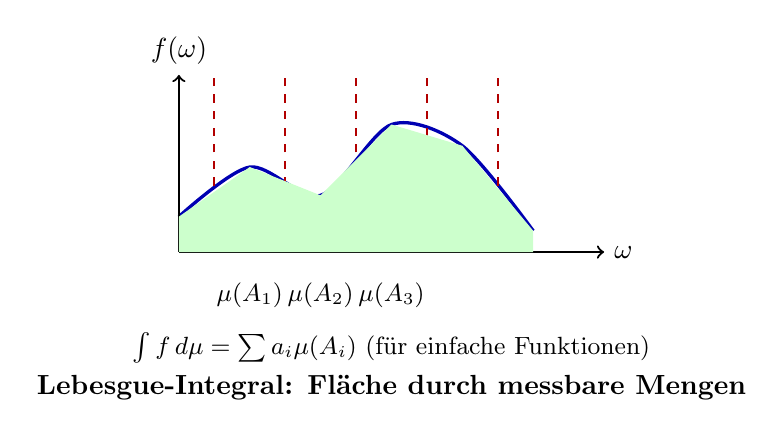
\begin{tikzpicture}[scale=0.9]
    % Funktion f
    \draw[blue!70!black, very thick, smooth] plot coordinates {(0,0.5) (1,1.2) (2,0.8) (3,1.8) (4,1.5) (5,0.3)};
    
    % x-Achse
    \draw[->, thick] (0,0) -- (6,0) node[right] {$\omega$};
    \draw[->, thick] (0,0) -- (0,2.5) node[above] {$f(\omega)$};
    
    % Messbare Mengen (nicht Rechtecke!)
    \draw[red!70!black, dashed, thick] (0.5,0) -- (0.5,2.5);
    \draw[red!70!black, dashed, thick] (1.5,0) -- (1.5,2.5);
    \draw[red!70!black, dashed, thick] (2.5,0) -- (2.5,2.5);
    \draw[red!70!black, dashed, thick] (3.5,0) -- (3.5,2.5);
    \draw[red!70!black, dashed, thick] (4.5,0) -- (4.5,2.5);
    
    % Fläche unter Kurve (approximiert durch messbare Mengen)
    \fill[green!20] (0,0) -- (0,0.5) -- (1,1.2) -- (2,0.8) -- (3,1.8) -- (4,1.5) -- (5,0.3) -- (5,0) -- cycle;
    
    % Maß-Werte
    \node[below] at (1, -0.3) {\small $\mu(A_1)$};
    \node[below] at (2, -0.3) {\small $\mu(A_2)$};
    \node[below] at (3, -0.3) {\small $\mu(A_3)$};
    
    % Integral-Formel
    \node[below] at (3, -1) {\small $\int f \, d\mu = \sum a_i \mu(A_i)$ (für einfache Funktionen)};
    
    % Label
    \node[below] at (3, -1.6) {\textbf{Lebesgue-Integral: Fläche durch messbare Mengen}};
\end{tikzpicture}
\end{center}
\end{denoobification}

\begin{denoobification}[Wichtige Konvergenzsätze]
\textbf{Monotoner Konvergenzsatz:}
Wenn $0 \leq f_1 \leq f_2 \leq \cdots$ messbare Funktionen sind und $f_n \to f$ punktweise, dann:
\[
\lim_{n \to \infty} \int f_n \, d\mu = \int f \, d\mu
\]

\textbf{Dominierte Konvergenzsatz (Satz von Lebesgue):}
Wenn $f_n \to f$ punktweise und $|f_n| \leq g$ für eine integrierbare Funktion $g$, dann:
\[
\lim_{n \to \infty} \int f_n \, d\mu = \int f \, d\mu
\]

\textbf{Fatou's Lemma:}
Für nicht-negative messbare Funktionen $f_n$:
\[
\int \liminf_{n \to \infty} f_n \, d\mu \leq \liminf_{n \to \infty} \int f_n \, d\mu
\]

\textbf{Intuition:} Diese Sätze erlauben es, Grenzwerte und Integrale zu vertauschen - essentiell für die Stochastische Calculus!

\textbf{Industrielle Anwendung (Elektrotechnik/Informatik):}
\begin{itemize}
    \item \textbf{Filter-Konvergenz:} Bei adaptiven Filtern konvergiert die Filterantwort: $\lim_{n \to \infty} \int H_n(f) S(f) df = \int \lim_{n \to \infty} H_n(f) S(f) df$ (Monotoner Konvergenzsatz)
    \item \textbf{Signal-Rekonstruktion:} Bei der Approximation von Signalen durch Fourier-Reihen: $\lim_{N \to \infty} \int s_N(t) dt = \int \lim_{N \to \infty} s_N(t) dt$
    \item \textbf{Adaptive Systeme:} In der Regelungstechnik konvergieren adaptive Algorithmen - der Dominierte Konvergenzsatz garantiert, dass Grenzwert und Integration vertauscht werden können
    \item \textbf{Monte-Carlo-Simulation:} Bei der numerischen Integration konvergieren Monte-Carlo-Schätzungen: $\lim_{N \to \infty} \frac{1}{N}\sum_{i=1}^N f(X_i) = \int f(x) d\mathbb{P}(x)$
\end{itemize}

\textbf{Mars-Kolonisierung Anwendung:}
\begin{itemize}
    \item \textbf{Adaptive Lebenserhaltungssysteme:} Bei adaptiven Systemen konvergieren Regelungsalgorithmen: $\lim_{n \to \infty} \int \text{Regelung}_n(t) dt = \int \lim_{n \to \infty} \text{Regelung}_n(t) dt$ - System lernt optimale Parameter
    \item \textbf{Ressourcen-Schätzung:} Monte-Carlo-Simulationen konvergieren bei der Schätzung von Ressourcen: $\lim_{N \to \infty} \frac{1}{N}\sum_{i=1}^N \text{Ressource}(X_i) = \int \text{Ressource}(x) d\mathbb{P}(x)$
    \item \textbf{Klima-Modellierung:} Bei der Approximation von Klimamodellen konvergieren iterative Verfahren - wichtig für Langzeitprognosen
    \item \textbf{Landungs-Simulation:} Monte-Carlo-Simulationen für Landungsmanöver konvergieren - ermöglicht Risikoabschätzung vor der Mission
\end{itemize}

\textbf{$\star$ Mental Model zum Auswendiglernen:}
\begin{itemize}
    \item \textbf{Analogie:} Konvergenzsätze sind wie "Tauschregeln" - wann können wir Grenzwert und Integral vertauschen?
    \item \textbf{Merksatz:} "Monotoner Konvergenzsatz = wachsende Funktionen → Grenzwert = Integral des Grenzwerts"
    \item \textbf{Merksatz:} "Dominierter Konvergenzsatz = beschränkte Funktionen → Grenzwert = Integral des Grenzwerts"
    \item \textbf{Visualisierung:} Wie ein "Tauschgeschäft" - unter bestimmten Bedingungen können Sie Grenzwert und Integral tauschen
\end{itemize}

\begin{center}
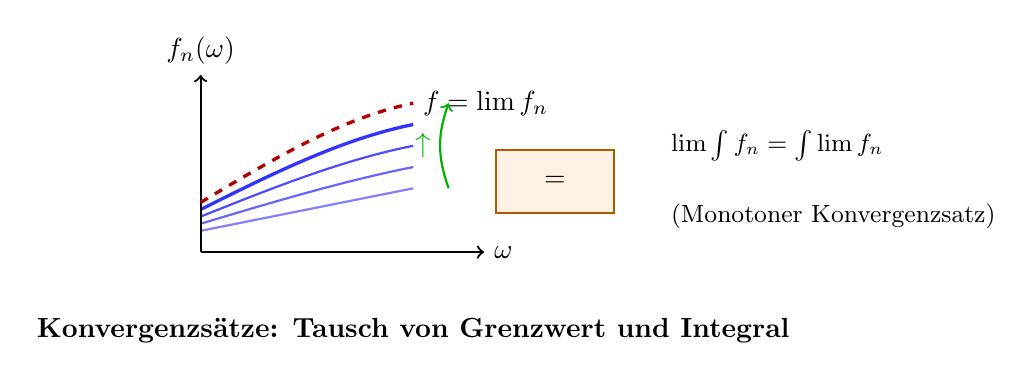
\begin{tikzpicture}[scale=0.9]
    % Funktionenfolge f_n
    \draw[blue!50, thick] (0,0.3) .. controls (1,0.5) and (2,0.7) .. (3,0.9);
    \draw[blue!60, thick] (0,0.4) .. controls (1,0.7) and (2,1) .. (3,1.2);
    \draw[blue!70, thick] (0,0.5) .. controls (1,0.9) and (2,1.3) .. (3,1.5);
    \draw[blue!80, very thick] (0,0.6) .. controls (1,1.1) and (2,1.6) .. (3,1.8);
    
    % x-Achse
    \draw[->, thick] (0,0) -- (4,0) node[right] {$\omega$};
    \draw[->, thick] (0,0) -- (0,2.5) node[above] {$f_n(\omega)$};
    
    % Grenzfunktion f
    \draw[red!70!black, very thick, dashed] (0,0.7) .. controls (1,1.3) and (2,1.9) .. (3,2.1);
    \node[right] at (3, 2.1) {$f = \lim f_n$};
    
    % Pfeile zeigen Konvergenz
    \draw[->, thick, green!70!black] (3.5, 0.9) to[bend left=20] node[above, sloped] {$\to$} (3.5, 2.1);
    
    % Gleichheitszeichen
    \node[rectangle, draw=orange!70!black, thick, minimum width=1.5cm, minimum height=0.8cm, fill=orange!10] (equal) at (5, 1) {};
    \node at (5, 1) {$=$};
    
    % Integral-Gleichung
    \node[right] at (6.5, 1.5) {\small $\lim \int f_n = \int \lim f_n$};
    \node[right] at (6.5, 0.5) {\small (Monotoner Konvergenzsatz)};
    
    % Label
    \node[below] at (3, -0.8) {\textbf{Konvergenzsätze: Tausch von Grenzwert und Integral}};
\end{tikzpicture}
\end{center}
\end{denoobification}

\section{Produktmaße und Fubini}

\begin{denoobification}[Produkt-$\sigma$-Algebra]
\textbf{Was ist eine Produkt-$\sigma$-Algebra?}

Für messbare Räume $(\Omega_1, \mathcal{F}_1)$ und $(\Omega_2, \mathcal{F}_2)$ ist die \textbf{Produkt-$\sigma$-Algebra} $\mathcal{F}_1 \otimes \mathcal{F}_2$ die kleinste $\sigma$-Algebra auf $\Omega_1 \times \Omega_2$, die alle "Rechtecke" $A_1 \times A_2$ mit $A_1 \in \mathcal{F}_1$, $A_2 \in \mathcal{F}_2$ enthält.

\textbf{Intuition:} Die Produkt-$\sigma$-Algebra beschreibt "gemeinsame Ereignisse" in zwei Räumen.

\textbf{Beispiel:} Bei zwei Würfeln ist $\Omega = \{1, \ldots, 6\} \times \{1, \ldots, 6\}$ und $\mathcal{F}$ enthält alle Kombinationen.

\textbf{Industrielle Anwendung (Elektrotechnik/Informatik):}
\begin{itemize}
    \item \textbf{MIMO-Systeme:} In der drahtlosen Kommunikation beschreibt $\mathcal{F}_1 \otimes \mathcal{F}_2$ die gemeinsamen Ereignisse von Sende- und Empfangsantennen - jede Antenne hat ihre eigene $\sigma$-Algebra
    \item \textbf{Mehrkanal-Signalverarbeitung:} Bei Stereo-Audio oder Mehrkanal-Sensoren beschreibt die Produkt-$\sigma$-Algebra alle möglichen Kombinationen von Signalen aus verschiedenen Kanälen
    \item \textbf{Sensor-Arrays:} Bei einem Array von Sensoren (z.B. Beschleunigungssensoren in verschiedenen Richtungen) beschreibt die Produkt-$\sigma$-Algebra alle möglichen Kombinationen von Messwerten
\end{itemize}

\textbf{Mars-Kolonisierung Anwendung:}
\begin{itemize}
    \item \textbf{Multi-Habitat-Systeme:} Die Produkt-$\sigma$-Algebra beschreibt alle möglichen Kombinationen von Zuständen in verschiedenen Habitaten - wichtig für Redundanz-Planung
    \item \textbf{Rover-Sensor-Arrays:} Bei einem Rover mit mehreren Sensoren (Kamera, Spektrometer, Bohrer) beschreibt die Produkt-$\sigma$-Algebra alle möglichen Kombinationen von Messwerten
    \item \textbf{Erd-Mars-Kommunikation:} Die Produkt-$\sigma$-Algebra beschreibt alle möglichen Kombinationen von Kommunikationszuständen (Erde-Seite $\times$ Mars-Seite) - kritisch für Missionskontrolle
\end{itemize}

\begin{center}
\begin{tikzpicture}[scale=0.9]
    % Omega 1
    \node[ellipse, draw=blue!70!black, thick, minimum width=2.5cm, minimum height=1.5cm, fill=blue!5] (omega1) at (0,0) {$\Omega_1$};
    
    % Omega 2
    \node[ellipse, draw=green!70!black, thick, minimum width=2.5cm, minimum height=1.5cm, fill=green!5] (omega2) at (5,0) {$\Omega_2$};
    
    % Produktraum
    \node[rectangle, draw=red!70!black, thick, minimum width=3cm, minimum height=2cm, fill=red!5] (product) at (2.5, 3) {$\Omega_1 \times \Omega_2$};
    
    % Rechtecke A1 x A2
    \draw[orange!70!black, dashed, very thick] (1, 2.5) rectangle (2, 3.5);
    \node[above] at (1.5, 3.5) {\small $A_1 \times A_2$};
    
    % Pfeile
    \draw[->, thick, blue!70!black] (omega1) to[bend left=30] node[above, sloped] {$A_1 \in \mathcal{F}_1$} (1.5, 2.5);
    \draw[->, thick, green!70!black] (omega2) to[bend right=30] node[below, sloped] {$A_2 \in \mathcal{F}_2$} (3.5, 2.5);
    
    % Produkt-sigma-Algebra
    \node[below] at (2.5, 1.5) {\small $\mathcal{F}_1 \otimes \mathcal{F}_2 = \sigma(\{A_1 \times A_2 : A_1 \in \mathcal{F}_1, A_2 \in \mathcal{F}_2\})$};
    
    % Label
    \node[below] at (2.5, 0.8) {\textbf{Produkt-$\sigma$-Algebra: Rechtecke $A_1 \times A_2$}};
\end{tikzpicture}
\end{center}
\end{denoobification}

\begin{denoobification}[Produktmaß]
\textbf{Was ist ein Produktmaß?}

Für Maße $\mu_1$ auf $(\Omega_1, \mathcal{F}_1)$ und $\mu_2$ auf $(\Omega_2, \mathcal{F}_2)$ ist das \textbf{Produktmaß} $\mu_1 \otimes \mu_2$ auf $(\Omega_1 \times \Omega_2, \mathcal{F}_1 \otimes \mathcal{F}_2)$ definiert durch:
\[
(\mu_1 \otimes \mu_2)(A_1 \times A_2) = \mu_1(A_1) \cdot \mu_2(A_2)
\]

\textbf{Intuition:} Das Produktmaß beschreibt "unabhängige" Maße auf dem Produktraum.

\textbf{$\star$ Mental Model zum Auswendiglernen:}
\begin{itemize}
    \item \textbf{Analogie:} Produktmaß = "Multiplikation von Maßen" - wie Fläche = Länge × Breite
    \item \textbf{Merksatz:} "Produktmaß = Maß von Rechteck = Maß(Seite 1) × Maß(Seite 2)"
    \item \textbf{Visualisierung:} Wie ein "Kartesisches Produkt" - für jedes Paar $(a,b)$ ist das Maß $\mu_1(a) \times \mu_2(b)$
\end{itemize}

\textbf{In der Wahrscheinlichkeit:} Wenn $X$ und $Y$ unabhängig sind, dann ist $\mathbb{P}_{(X,Y)} = \mathbb{P}_X \otimes \mathbb{P}_Y$.

\textbf{Industrielle Anwendung (Elektrotechnik/Informatik):}
\begin{itemize}
    \item \textbf{Unabhängige Kanäle:} In der Kommunikationstechnik sind zwei Kanäle unabhängig, wenn $\mathbb{P}(\text{Fehler in Kanal 1 und 2}) = \mathbb{P}(\text{Fehler in Kanal 1}) \times \mathbb{P}(\text{Fehler in Kanal 2})$
    \item \textbf{Parallel-Systeme:} Bei redundanten Systemen (z.B. zwei unabhängige Prozessoren) ist die Ausfallwahrscheinlichkeit das Produkt der Einzelwahrscheinlichkeiten
    \item \textbf{Unabhängige Sensoren:} Wenn zwei Sensoren unabhängig messen (z.B. Temperatur und Druck), ist die gemeinsame Verteilung das Produkt der Einzelverteilungen
    \item \textbf{Rauschen in verschiedenen Frequenzbändern:} Weißes Rauschen in verschiedenen Bändern ist unabhängig - die gemeinsame Verteilung ist das Produktmaß
\end{itemize}

\textbf{Mars-Kolonisierung Anwendung:}
\begin{itemize}
    \item \textbf{Redundante Lebenserhaltungssysteme:} Wenn zwei unabhängige Systeme vorhanden sind, ist die Ausfallwahrscheinlichkeit: $\mathbb{P}(\text{beide ausfallen}) = \mathbb{P}(\text{System 1 ausfällt}) \times \mathbb{P}(\text{System 2 ausfällt})$ - bestimmt Sicherheitsmargen
    \item \textbf{Unabhängige Ressourcenquellen:} Wenn Wasser aus zwei unabhängigen Quellen gewonnen wird, ist die gemeinsame Verfügbarkeit das Produkt der Einzelverfügbarkeiten
    \item \textbf{Multi-Rover-Missionen:} Wenn mehrere Rover unabhängig operieren, ist die gemeinsame Erfolgswahrscheinlichkeit das Produkt der Einzelerfolgswahrscheinlichkeiten
    \item \textbf{Unabhängige Kommunikationswege:} Wenn mehrere Kommunikationswege unabhängig sind, ist die Wahrscheinlichkeit eines totalen Kommunikationsverlusts das Produkt der Einzelwahrscheinlichkeiten
\end{itemize}

\textbf{$\star$ Mental Model zum Auswendiglernen:}
\begin{itemize}
    \item \textbf{Analogie:} Produktmaß = "Multiplikation von Maßen" - wie Fläche = Länge × Breite
    \item \textbf{Merksatz:} "Produktmaß = Maß von Rechteck = Maß(Seite 1) × Maß(Seite 2)"
    \item \textbf{Visualisierung:} Wie ein "Kartesisches Produkt" - für jedes Paar $(a,b)$ ist das Maß $\mu_1(a) \times \mu_2(b)$
\end{itemize}

\begin{center}
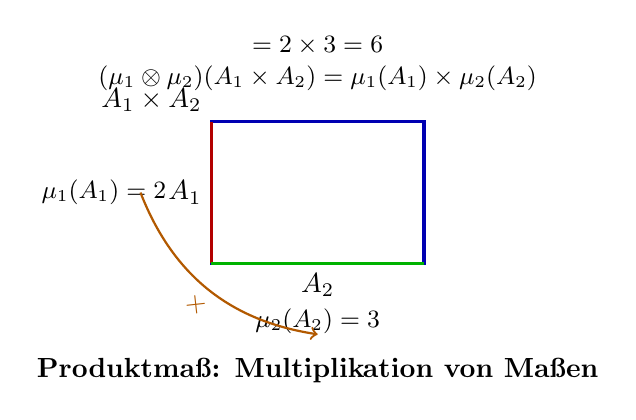
\begin{tikzpicture}[scale=0.9]
    % Rechteck A1 x A2
    \draw[blue!70!black, very thick] (0,0) rectangle (3,2);
    \node[above left] at (0,2) {$A_1 \times A_2$};
    
    % Seiten markieren
    \draw[red!70!black, very thick] (0,0) -- (0,2);
    \node[left] at (0,1) {$A_1$};
    \draw[green!70!black, very thick] (0,0) -- (3,0);
    \node[below] at (1.5, 0) {$A_2$};
    
    % Maß-Werte
    \node[left] at (-0.5, 1) {\small $\mu_1(A_1) = 2$};
    \node[below] at (1.5, -0.5) {\small $\mu_2(A_2) = 3$};
    
    % Produktmaß
    \node[above] at (1.5, 2.3) {\small $(\mu_1 \otimes \mu_2)(A_1 \times A_2) = \mu_1(A_1) \times \mu_2(A_2)$};
    \node[above] at (1.5, 2.8) {\small $= 2 \times 3 = 6$};
    
    % Multiplikations-Symbol
    \draw[->, thick, orange!70!black] (-1, 1) to[bend right=30] node[below, sloped] {$\times$} (1.5, -1);
    
    % Label
    \node[below] at (1.5, -1.2) {\textbf{Produktmaß: Multiplikation von Maßen}};
\end{tikzpicture}
\end{center}
\end{denoobification}

\begin{denoobification}[Satz von Fubini]
\textbf{Was besagt der Satz von Fubini?}

Der \textbf{Satz von Fubini} erlaubt es, Integrale über Produkträume als iterierte Integrale zu berechnen:

\[
\int_{\Omega_1 \times \Omega_2} f(\omega_1, \omega_2) \, d(\mu_1 \otimes \mu_2) = \int_{\Omega_1} \left(\int_{\Omega_2} f(\omega_1, \omega_2) \, d\mu_2(\omega_2)\right) d\mu_1(\omega_1)
\]

\textbf{Intuition:} Man kann "von innen nach außen" integrieren.

\textbf{Beispiel:} Für $f(x,y) = xy$ auf $[0,1] \times [0,1]$:
\[
\int_0^1 \int_0^1 xy \, dx \, dy = \int_0^1 x \, dx \cdot \int_0^1 y \, dy = \frac{1}{2} \cdot \frac{1}{2} = \frac{1}{4}
\]

\textbf{Warum wichtig?} Essentiell für bedingte Erwartungen und mehrdimensionale Integration!

\textbf{Industrielle Anwendung (Elektrotechnik/Informatik):}
\begin{itemize}
    \item \textbf{2D-Signalverarbeitung:} Bei Bildverarbeitung kann die Leistung über ein 2D-Frequenzband berechnet werden: $\iint |H(f_x, f_y)|^2 S(f_x, f_y) df_x df_y = \int \left(\int |H|^2 S df_y\right) df_x$
    \item \textbf{Mehrdimensionale Filter:} Bei der Filterung von mehrdimensionalen Signalen (z.B. Video) erlaubt Fubini die Berechnung als iterierte eindimensionale Filterung
    \item \textbf{Spektralanalyse:} Die Berechnung des Leistungsspektrums über Zeit und Frequenz: $\iint W(t,f) dt df = \int \left(\int W(t,f) dt\right) df$
    \item \textbf{Optimierung:} Bei der Optimierung von Systemparametern über mehrere Dimensionen kann Fubini die Berechnung vereinfachen
\end{itemize}

\textbf{Mars-Kolonisierung Anwendung:}
\begin{itemize}
    \item \textbf{3D-Ressourcen-Kartierung:} Die Berechnung von Ressourcen über Raum und Zeit: $\iiint \text{Ressource}(x,y,t) dx dy dt = \int \left(\int \left(\int \text{Ressource} dt\right) dy\right) dx$ - wichtig für Erkundungsplanung
    \item \textbf{Habitat-Klima-Modellierung:} Die Berechnung von Klimaparametern über Raum und Zeit kann als iterierte Integration erfolgen - vereinfacht numerische Berechnungen
    \item \textbf{Rover-Trajektorien-Optimierung:} Die Optimierung von Rover-Routen über Raum und Zeit kann durch Fubini vereinfacht werden
    \item \textbf{Energie-Verteilung:} Die Berechnung der Energieverteilung über verschiedene Systeme und Zeit: $\iint E(\text{System}, t) d\text{System} dt$ - wichtig für Energie-Management
\end{itemize}

\textbf{$\star$ Mental Model zum Auswendiglernen:}
\begin{itemize}
    \item \textbf{Analogie:} Fubini = "von innen nach außen integrieren" - wie beim Schälen einer Zwiebel
    \item \textbf{Merksatz:} "Fubini = mehrdimensionales Integral = iteriertes eindimensionales Integral"
    \item \textbf{Visualisierung:} Wie ein "Schichten-Kuchen" - integrieren Sie zuerst über eine Dimension, dann über die andere
\end{itemize}

\begin{center}
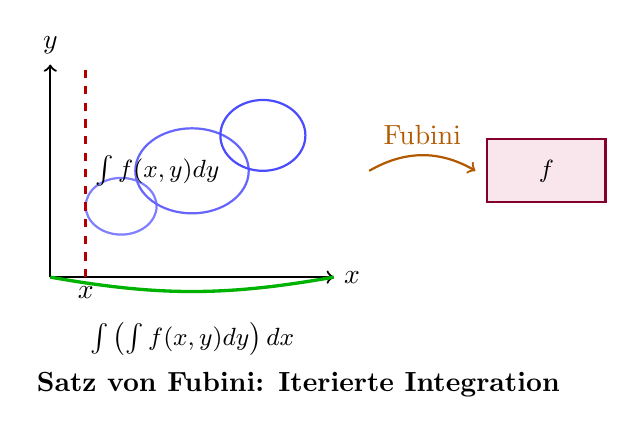
\begin{tikzpicture}[scale=0.9]
    % 2D-Funktion f(x,y)
    \draw[->, thick] (0,0) -- (4,0) node[right] {$x$};
    \draw[->, thick] (0,0) -- (0,3) node[above] {$y$};
    
    % Kontur-Linien
    \draw[blue!50, thick] (1,1) ellipse (0.5cm and 0.4cm);
    \draw[blue!60, thick] (2,1.5) ellipse (0.8cm and 0.6cm);
    \draw[blue!70, thick] (3,2) ellipse (0.6cm and 0.5cm);
    
    % Iterierte Integration: zuerst über y
    \draw[red!70!black, dashed, very thick] (0.5,0) -- (0.5,3);
    \node[below] at (0.5, 0) {$x$};
    \node[right] at (0.5, 1.5) {\small $\int f(x,y) dy$};
    
    % Dann über x
    \draw[green!70!black, very thick] (0,0) to[bend right=10] (4,0);
    \node[below] at (2, -0.5) {\small $\int \left(\int f(x,y) dy\right) dx$};
    
    % Pfeil zeigt Prozess
    \draw[->, thick, orange!70!black] (4.5, 1.5) to[bend left=30] node[above, sloped] {Fubini} (6, 1.5);
    
    % Ergebnis
    \node[rectangle, draw=purple!70!black, thick, minimum width=1.5cm, minimum height=0.8cm, fill=purple!10] (result) at (7, 1.5) {};
    \node at (7, 1.5) {\small $\iint f$};
    
    % Label
    \node[below] at (3.5, -1.2) {\textbf{Satz von Fubini: Iterierte Integration}};
\end{tikzpicture}
\end{center}
\end{denoobification}

\section{Gemeinsame und Randdichten}

\begin{denoobification}[Gemeinsame Dichte (Joint Density)]
\textbf{Was ist eine gemeinsame Dichte?}

Für zwei Zufallsvariablen $X$ und $Y$ ist die \textbf{gemeinsame Dichte} $f_{X,Y}(x,y)$ die Dichte der gemeinsamen Verteilung $\mathbb{P}_{(X,Y)}$ bezüglich des Produktmaßes.

\textbf{Formale Definition:}
\[
\mathbb{P}(X \in A, Y \in B) = \int_A \int_B f_{X,Y}(x,y) \, dy \, dx
\]

\textbf{Intuition:} Die gemeinsame Dichte beschreibt, wie wahrscheinlich es ist, dass $X$ und $Y$ gleichzeitig bestimmte Werte annehmen.

\textbf{Eigenschaften:}
\begin{itemize}
    \item \textbf{Nicht-Negativität:} $f_{X,Y}(x,y) \geq 0$ für alle $x, y$
    \item \textbf{Normierung:} $\int_{-\infty}^{\infty} \int_{-\infty}^{\infty} f_{X,Y}(x,y) \, dx \, dy = 1$
    \item \textbf{Wahrscheinlichkeiten:} $\mathbb{P}((X,Y) \in D) = \iint_D f_{X,Y}(x,y) \, dx \, dy$ für jede Region $D$
\end{itemize}

\textbf{Beispiele:}
\begin{itemize}
    \item \textbf{Unabhängige Zufallsvariablen:} $f_{X,Y}(x,y) = f_X(x) \cdot f_Y(y)$
    \item \textbf{Bivariate Normalverteilung:} $f_{X,Y}(x,y) = \frac{1}{2\pi\sigma_X\sigma_Y\sqrt{1-\rho^2}} \exp\left(-\frac{1}{2(1-\rho^2)}\left[\frac{(x-\mu_X)^2}{\sigma_X^2} - \frac{2\rho(x-\mu_X)(y-\mu_Y)}{\sigma_X\sigma_Y} + \frac{(y-\mu_Y)^2}{\sigma_Y^2}\right]\right)$
\end{itemize}

\textbf{Industrielle Anwendung (Elektrotechnik/Informatik):}
\begin{itemize}
    \item \textbf{Korrelationsanalyse:} In der Signalverarbeitung beschreibt $f_{X,Y}(x,y)$ die gemeinsame Verteilung von zwei korrelierten Signalen (z.B. Eingangs- und Ausgangssignal eines Systems)
    \item \textbf{Sensor-Kalibrierung:} Bei der Kalibrierung von zwei Sensoren beschreibt die gemeinsame Dichte die Wahrscheinlichkeit bestimmter Kombinationen von Messwerten
    \item \textbf{Kanal-Modellierung:} In der Kommunikationstechnik beschreibt $f_{X,Y}$ die gemeinsame Verteilung von gesendetem ($X$) und empfangenem ($Y$) Signal bei Rauschen
    \item \textbf{Feature-Korrelation:} In der Mustererkennung beschreibt die gemeinsame Dichte die Korrelation zwischen verschiedenen Features (z.B. Frequenz und Amplitude)
\end{itemize}

\textbf{Mars-Kolonisierung Anwendung:}
\begin{itemize}
    \item \textbf{Temperatur-Druck-Korrelation:} $f_{X,Y}(T,P)$ beschreibt die gemeinsame Verteilung von Temperatur und Druck im Habitat - wichtig für Klimakontrolle
    \item \textbf{Sauerstoff-CO$_2$-Korrelation:} Die gemeinsame Dichte beschreibt die Korrelation zwischen Sauerstoff- und CO$_2$-Konzentration - kritisch für Atmosphären-Management
    \item \textbf{Energie-Verbrauch-Korrelation:} $f_{X,Y}(E_{\text{verfügbar}}, E_{\text{verbraucht}})$ beschreibt die gemeinsame Verteilung - wichtig für Energie-Planung
    \item \textbf{Ressourcen-Korrelation:} Die gemeinsame Dichte beschreibt die Korrelation zwischen verschiedenen Ressourcen (z.B. Wasser und Energie für Elektrolyse) - wichtig für Produktionsplanung
\end{itemize}

\textbf{$\star$ Mental Model zum Auswendiglernen:}
\begin{itemize}
    \item \textbf{Analogie:} Gemeinsame Dichte = "3D-Landschaft" - zeigt Wahrscheinlichkeit für jedes Paar $(x,y)$
    \item \textbf{Merksatz:} "Gemeinsame Dichte = Dichte von $(X,Y)$ zusammen"
    \item \textbf{Visualisierung:} Wie ein "Gebirge" - hohe Werte = wahrscheinliche Kombinationen, niedrige Werte = unwahrscheinliche Kombinationen
    \item \textbf{Integration:} Fläche unter der Dichte über einer Region = Wahrscheinlichkeit
\end{itemize}

\begin{center}
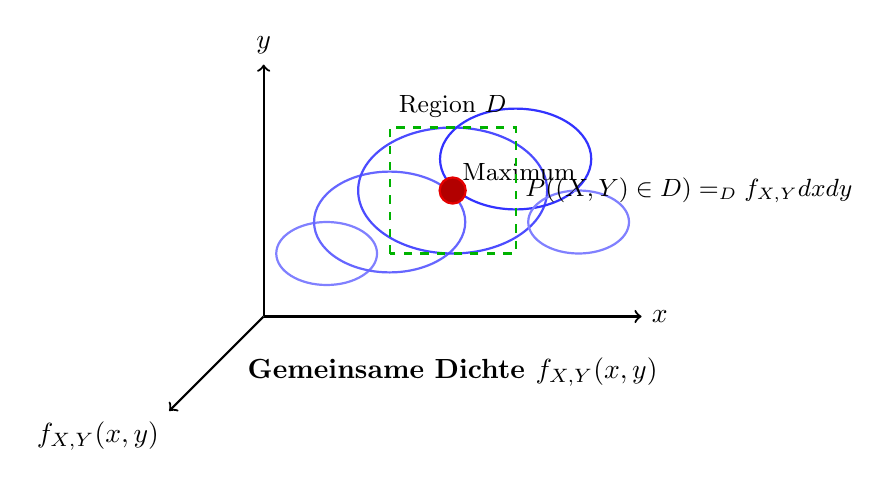
\begin{tikzpicture}[scale=0.8]
    % 3D-ähnliche Darstellung der gemeinsamen Dichte
    \draw[->, thick] (0,0) -- (6,0) node[right] {$x$};
    \draw[->, thick] (0,0) -- (0,4) node[above] {$y$};
    \draw[->, thick] (0,0) -- (-1.5,-1.5) node[below left] {$f_{X,Y}(x,y)$};
    
    % Kontur-Linien (Höhenlinien)
    \draw[blue!50, thick] (1,1) ellipse (0.8cm and 0.5cm);
    \draw[blue!60, thick] (2,1.5) ellipse (1.2cm and 0.8cm);
    \draw[blue!70, thick] (3,2) ellipse (1.5cm and 1cm);
    \draw[blue!80, thick] (4,2.5) ellipse (1.2cm and 0.8cm);
    \draw[blue!50, thick] (5,1.5) ellipse (0.8cm and 0.5cm);
    
    % Zentrum (Maximum)
    \node[circle, fill=red!70!black, draw=red!90!black, thick, minimum size=0.3cm] at (3,2) {};
    \node[above right] at (3,2) {\small Maximum};
    
    % Region markieren
    \draw[green!70!black, dashed, thick] (2,1) rectangle (4,3);
    \node[above] at (3,3) {\small Region $D$};
    \node[right] at (4,2) {\small $\mathbb{P}((X,Y) \in D) = \iint_D f_{X,Y} dx dy$};
    
    % Label
    \node[below] at (3, -0.5) {\textbf{Gemeinsame Dichte $f_{X,Y}(x,y)$}};
\end{tikzpicture}
\end{center}
\end{denoobification}

\begin{denoobification}[Randdichten (Marginal Densities)]
\textbf{Was sind Randdichten?}

Die \textbf{Randdichte} einer Zufallsvariable ist die Dichte ihrer einzelnen Verteilung, erhalten durch "Integration über die andere Variable".

\textbf{Definition:}
\begin{align}
f_X(x) &= \int_{-\infty}^{\infty} f_{X,Y}(x,y) \, dy \quad \text{(Randdichte von $X$)} \\
f_Y(y) &= \int_{-\infty}^{\infty} f_{X,Y}(x,y) \, dx \quad \text{(Randdichte von $Y$)}
\end{align}

\textbf{Intuition:} Die Randdichte "projiziert" die gemeinsame Dichte auf eine Dimension - sie ignoriert die andere Variable.

\textbf{Interpretation:}
\begin{itemize}
    \item $f_X(x)$ beschreibt die Verteilung von $X$ allein (ohne Information über $Y$)
    \item $f_Y(y)$ beschreibt die Verteilung von $Y$ allein (ohne Information über $X$)
    \item Man "summiert" (integriert) über alle möglichen Werte der anderen Variable
\end{itemize}

\textbf{Beispiel:} Für bivariate Normalverteilung:
\begin{itemize}
    \item $f_X(x) = \frac{1}{\sigma_X\sqrt{2\pi}} \exp\left(-\frac{(x-\mu_X)^2}{2\sigma_X^2}\right)$ (Normalverteilung)
    \item $f_Y(y) = \frac{1}{\sigma_Y\sqrt{2\pi}} \exp\left(-\frac{(y-\mu_Y)^2}{2\sigma_Y^2}\right)$ (Normalverteilung)
\end{itemize}

\textbf{Industrielle Anwendung (Elektrotechnik/Informatik):}
\begin{itemize}
    \item \textbf{Einzelkanal-Analyse:} In der Signalverarbeitung beschreibt $f_X(x)$ die Verteilung eines Signals allein, ohne Berücksichtigung eines anderen Signals (z.B. nur Frequenz, ohne Phase)
    \item \textbf{Sensor-Charakterisierung:} Die Randdichte eines Sensors beschreibt seine Verteilung, wenn er isoliert betrachtet wird (ohne Korrelation mit anderen Sensoren)
    \item \textbf{Feature-Extraktion:} In der Mustererkennung beschreibt die Randdichte die Verteilung eines einzelnen Features (z.B. nur Helligkeit, ohne Farbe)
    \item \textbf{Rauschanalyse:} Die Randdichte beschreibt die Verteilung von Rauschen in einem einzelnen Kanal, unabhängig von anderen Kanälen
\end{itemize}

\textbf{Mars-Kolonisierung Anwendung:}
\begin{itemize}
    \item \textbf{Einzelparameter-Analyse:} $f_X(x)$ beschreibt die Verteilung eines einzelnen Parameters (z.B. nur Temperatur, ohne Druck) - wichtig für isolierte Systemanalyse
    \item \textbf{Ressourcen-Einzelanalyse:} Die Randdichte beschreibt die Verteilung einer einzelnen Ressource (z.B. nur Wasser, ohne Energie) - wichtig für Ressourcen-Planung
    \item \textbf{System-Isolation:} Die Randdichte beschreibt die Verteilung eines Systems, wenn es isoliert betrachtet wird (z.B. nur Lebenserhaltung, ohne Kommunikation) - wichtig für Fehleranalyse
    \item \textbf{Kolonist-Gesundheit:} Die Randdichte beschreibt die Verteilung eines einzelnen Gesundheitsparameters (z.B. nur Strahlungsdosis, ohne Ernährung) - wichtig für medizinische Überwachung
\end{itemize}

\textbf{$\star$ Mental Model zum Auswendiglernen:}
\begin{itemize}
    \item \textbf{Analogie:} Randdichte = "Schatten" der gemeinsamen Dichte - projiziert auf eine Achse
    \item \textbf{Merksatz:} "Randdichte = Integration über andere Variable"
    \item \textbf{Visualisierung:} Wie ein "Schattenwurf" - die 3D-Landschaft wirft einen Schatten auf die $x$- oder $y$-Achse
    \item \textbf{Prozess:} "Vergessen" Sie eine Variable → integrieren Sie sie weg → erhalten Sie die Randdichte
\end{itemize}

\begin{center}
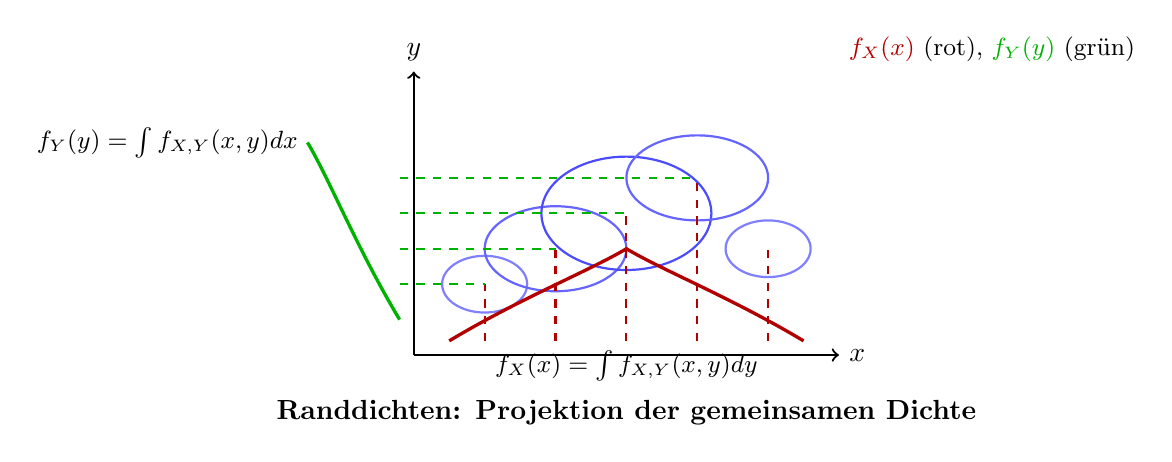
\begin{tikzpicture}[scale=0.9]
    % Gemeinsame Dichte (3D-Ansicht)
    \draw[->, thick] (0,0) -- (6,0) node[right] {$x$};
    \draw[->, thick] (0,0) -- (0,4) node[above] {$y$};
    
    % Kontur-Linien der gemeinsamen Dichte
    \draw[blue!50, thick] (1,1) ellipse (0.6cm and 0.4cm);
    \draw[blue!60, thick] (2,1.5) ellipse (1cm and 0.6cm);
    \draw[blue!70, thick] (3,2) ellipse (1.2cm and 0.8cm);
    \draw[blue!60, thick] (4,2.5) ellipse (1cm and 0.6cm);
    \draw[blue!50, thick] (5,1.5) ellipse (0.6cm and 0.4cm);
    
    % Randdichte f_X(x) - Projektion auf x-Achse
    \draw[red!70!black, very thick] (0.5,0.2) .. controls (1.5,0.8) and (2.5,1.2) .. (3,1.5) .. controls (3.5,1.2) and (4.5,0.8) .. (5.5,0.2);
    \node[below] at (3, 0.2) {\small $f_X(x) = \int f_{X,Y}(x,y) dy$};
    \draw[red!70!black, dashed, thick] (1,0.2) -- (1,1);
    \draw[red!70!black, dashed, thick] (2,0.2) -- (2,1.5);
    \draw[red!70!black, dashed, thick] (3,0.2) -- (3,2);
    \draw[red!70!black, dashed, thick] (4,0.2) -- (4,2.5);
    \draw[red!70!black, dashed, thick] (5,0.2) -- (5,1.5);
    
    % Randdichte f_Y(y) - Projektion auf y-Achse
    \draw[green!70!black, very thick] (-0.2,0.5) .. controls (-0.8,1.5) and (-1.2,2.5) .. (-1.5,3) .. controls (-1.2,2.5) and (-0.8,1.5) .. (-0.2,0.5);
    \node[left] at (-1.5, 3) {\small $f_Y(y) = \int f_{X,Y}(x,y) dx$};
    \draw[green!70!black, dashed, thick] (-0.2,1) -- (1,1);
    \draw[green!70!black, dashed, thick] (-0.2,1.5) -- (2,1.5);
    \draw[green!70!black, dashed, thick] (-0.2,2) -- (3,2);
    \draw[green!70!black, dashed, thick] (-0.2,2.5) -- (4,2.5);
    
    % Label
    \node[below] at (3, -0.5) {\textbf{Randdichten: Projektion der gemeinsamen Dichte}};
    \node[above right] at (6, 4) {\small \textcolor{red!70!black}{$f_X(x)$} (rot), \textcolor{green!70!black}{$f_Y(y)$} (grün)};
\end{tikzpicture}
\end{center}
\end{denoobification}

\begin{denoobification}[Bedingte Dichte (Conditional Density)]
\textbf{Was ist eine bedingte Dichte?}

Die \textbf{bedingte Dichte} $f_{Y|X}(y|x)$ beschreibt die Verteilung von $Y$ gegeben $X = x$.

\textbf{Definition:}
\[
f_{Y|X}(y|x) = \frac{f_{X,Y}(x,y)}{f_X(x)} \quad \text{wenn } f_X(x) > 0
\]

\textbf{Intuition:} Die bedingte Dichte ist die "Schnitt" durch die gemeinsame Dichte bei festem $x$, normiert durch die Randdichte.

\textbf{Eigenschaften:}
\begin{itemize}
    \item \textbf{Normierung:} $\int_{-\infty}^{\infty} f_{Y|X}(y|x) \, dy = 1$ für jedes $x$
    \item \textbf{Bayes' Regel:} $f_{X|Y}(x|y) = \frac{f_{Y|X}(y|x) f_X(x)}{f_Y(y)}$
    \item \textbf{Unabhängigkeit:} $X$ und $Y$ sind unabhängig genau dann, wenn $f_{Y|X}(y|x) = f_Y(y)$ für alle $x$
\end{itemize}

\textbf{Beispiel:} Für bivariate Normalverteilung:
\[
f_{Y|X}(y|x) = \frac{1}{\sigma_{Y|X}\sqrt{2\pi}} \exp\left(-\frac{(y - \mu_{Y|X})^2}{2\sigma_{Y|X}^2}\right)
\]
wobei $\mu_{Y|X} = \mu_Y + \rho \frac{\sigma_Y}{\sigma_X}(x - \mu_X)$ und $\sigma_{Y|X}^2 = \sigma_Y^2(1-\rho^2)$.

\textbf{Industrielle Anwendung (Elektrotechnik/Informatik):}
\begin{itemize}
    \item \textbf{Prädiktive Filterung:} In der Signalverarbeitung beschreibt $f_{Y|X}(y|x)$ die Verteilung des Ausgangssignals $Y$ gegeben das Eingangssignal $X = x$ - dies ist essentiell für prädiktive Filter
    \item \textbf{Kanal-Schätzung:} In der Kommunikationstechnik beschreibt die bedingte Dichte die Verteilung des empfangenen Signals gegeben das gesendete Signal - wichtig für Kanal-Schätzung und Equalizer
    \item \textbf{Adaptive Systeme:} Bei adaptiven Filtern wird die bedingte Verteilung verwendet, um das System an die Eingangsbedingungen anzupassen
    \item \textbf{Fehlerkorrektur:} In der Fehlerkorrektur beschreibt $f_{Y|X}$ die Wahrscheinlichkeit bestimmter Fehlermuster gegeben das gesendete Signal
    \item \textbf{Sensor-Fusion:} Bei der Fusion von Sensordaten beschreibt die bedingte Dichte die Verteilung eines Sensors gegeben die Werte anderer Sensoren
\end{itemize}

\textbf{Mars-Kolonisierung Anwendung:}
\begin{itemize}
    \item \textbf{Prädiktive Lebenserhaltung:} $f_{Y|X}(y|x)$ beschreibt die Verteilung des Systemzustands $Y$ gegeben die Eingangsparameter $X = x$ - wichtig für prädiktive Wartung
    \item \textbf{Erd-Kommunikation:} Die bedingte Dichte beschreibt die Verteilung des empfangenen Signals auf dem Mars gegeben das gesendete Signal von der Erde - wichtig für Signal-Rekonstruktion bei Störungen
    \item \textbf{Ressourcen-Vorhersage:} $f_{Y|X}$ beschreibt die Verteilung zukünftiger Ressourcen $Y$ gegeben aktuelle Bedingungen $X$ - wichtig für Langzeitplanung
    \item \textbf{Kolonist-Gesundheit:} Die bedingte Dichte beschreibt die Verteilung der Gesundheit $Y$ gegeben Umweltbedingungen $X$ (Strahlung, Druck, etc.) - kritisch für medizinische Überwachung
    \item \textbf{Landungs-Vorhersage:} $f_{Y|X}$ beschreibt die Verteilung des Landungserfolgs $Y$ gegeben Atmosphärenbedingungen $X$ - wichtig für Landungsmanöver
\end{itemize}

\textbf{$\star$ Mental Model zum Auswendiglernen:}
\begin{itemize}
    \item \textbf{Analogie:} Bedingte Dichte = "Schnitt" durch die gemeinsame Dichte bei festem $x$
    \item \textbf{Merksatz:} "$f_{Y|X}(y|x) = \frac{f_{X,Y}(x,y)}{f_X(x)}$ = gemeinsame geteilt durch Rand"
    \item \textbf{Visualisierung:} Wie ein "vertikaler Schnitt" durch die 3D-Landschaft bei $x = x_0$
    \item \textbf{Interpretation:} "Wenn ich weiß, dass $X = x$, wie ist dann $Y$ verteilt?"
\end{itemize}

\begin{center}
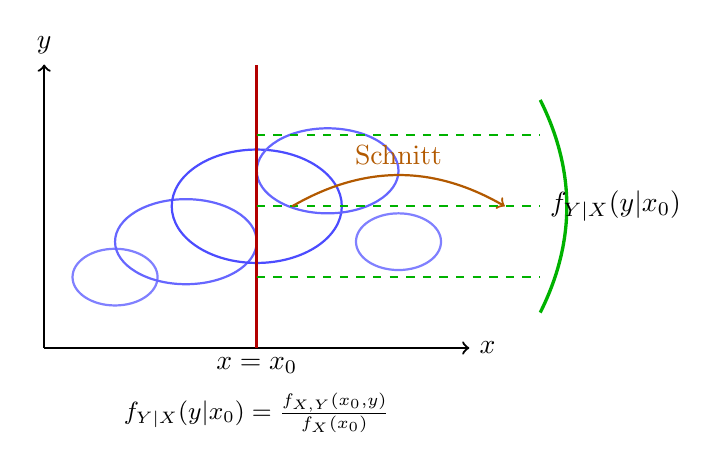
\begin{tikzpicture}[scale=0.9]
    % Gemeinsame Dichte
    \draw[->, thick] (0,0) -- (6,0) node[right] {$x$};
    \draw[->, thick] (0,0) -- (0,4) node[above] {$y$};
    
    % Kontur-Linien
    \draw[blue!50, thick] (1,1) ellipse (0.6cm and 0.4cm);
    \draw[blue!60, thick] (2,1.5) ellipse (1cm and 0.6cm);
    \draw[blue!70, thick] (3,2) ellipse (1.2cm and 0.8cm);
    \draw[blue!60, thick] (4,2.5) ellipse (1cm and 0.6cm);
    \draw[blue!50, thick] (5,1.5) ellipse (0.6cm and 0.4cm);
    
    % Vertikaler Schnitt bei x = 3
    \draw[red!70!black, very thick] (3,0) -- (3,4);
    \node[below] at (3, 0) {$x = x_0$};
    
    % Bedingte Dichte f_Y|X(y|x_0) - rechts
    \draw[green!70!black, very thick] (7,0.5) .. controls (7.5,1.5) and (7.5,2.5) .. (7,3.5);
    \node[right] at (7, 2) {$f_{Y|X}(y|x_0)$};
    \draw[green!70!black, dashed, thick] (3,1) -- (7,1);
    \draw[green!70!black, dashed, thick] (3,2) -- (7,2);
    \draw[green!70!black, dashed, thick] (3,3) -- (7,3);
    
    % Pfeil zeigt Transformation
    \draw[->, thick, orange!70!black] (3.5, 2) to[bend left=30] node[above] {Schnitt} (6.5, 2);
    
    % Formel
    \node[below] at (3, -0.5) {\small $f_{Y|X}(y|x_0) = \frac{f_{X,Y}(x_0,y)}{f_X(x_0)}$};
\end{tikzpicture}
\end{center}
\end{denoobification}

\section{Radon-Nikodym Theorem}

\begin{denoobification}[Absolute Stetigkeit]
\textbf{Was bedeutet absolute Stetigkeit?}

Ein Maß $\nu$ heißt \textbf{absolut stetig} bezüglich $\mu$ (geschrieben $\nu \ll \mu$), wenn für alle $A \in \mathcal{F}$ gilt:
\[
\mu(A) = 0 \Rightarrow \nu(A) = 0
\]

\textbf{Intuition:} $\nu$ "respektiert" die Nullmengen von $\mu$.

\textbf{Beispiel:} Jedes Wahrscheinlichkeitsmaß mit Dichte ist absolut stetig bezüglich des Lebesgue-Maßes.

\textbf{Industrielle Anwendung (Elektrotechnik/Informatik):}
\begin{itemize}
    \item \textbf{Störungsanalyse:} Wenn ein System störungsfrei ist ($\mu(A) = 0$), dann sollte auch das gestörte System keine Störung in $A$ haben ($\nu(A) = 0$) - wichtig für Robustheitsanalyse
    \item \textbf{Rauschen:} Wenn ein Signal in einem Frequenzband keine Energie hat ($\mu(A) = 0$), dann sollte auch das verrauschte Signal dort keine Energie haben - dies beschreibt "additives Rauschen"
    \item \textbf{Fehlerfortpflanzung:} In der Fehleranalyse bedeutet absolute Stetigkeit, dass Fehler nur dort auftreten können, wo das ursprüngliche Signal nicht null ist
    \item \textbf{Signal-Rekonstruktion:} Bei der Signalrekonstruktion bedeutet $\nu \ll \mu$, dass das rekonstruierte Signal die Nullstellen des Originals respektiert
\end{itemize}

\textbf{Mars-Kolonisierung Anwendung:}
\begin{itemize}
    \item \textbf{System-Robustheit:} Wenn ein System in einem Zustand $A$ keine Probleme hat ($\mu(A) = 0$), dann sollte auch das gestörte System dort keine Probleme haben ($\nu(A) = 0$) - wichtig für Fehlertoleranz
    \item \textbf{Ressourcen-Verfügbarkeit:} Wenn eine Ressource in einer Region $A$ nicht vorhanden ist ($\mu(A) = 0$), dann sollte auch die gestörte/verrauschte Messung dort keine Ressource anzeigen - wichtig für Erkundungsplanung
    \item \textbf{Kommunikations-Störungen:} Wenn ein Kommunikationskanal in einem Frequenzband keine Signale hat ($\mu(A) = 0$), dann sollte auch der gestörte Kanal dort keine Signale haben - beschreibt "additives Rauschen" in Erd-Mars-Kommunikation
    \item \textbf{Fehlerfortpflanzung in Systemen:} Absolute Stetigkeit bedeutet, dass Systemfehler nur dort auftreten können, wo das ursprüngliche System nicht perfekt funktioniert - wichtig für Redundanz-Planung
\end{itemize}

\textbf{$\star$ Mental Model zum Auswendiglernen:}
\begin{itemize}
    \item \textbf{Analogie:} Absolute Stetigkeit = "Respekt für Nullmengen" - wenn $\mu$ sagt "das ist nichts", dann sagt $\nu$ auch "das ist nichts"
    \item \textbf{Merksatz:} "$\nu \ll \mu$ = wenn $\mu(A) = 0$, dann $\nu(A) = 0$"
    \item \textbf{Visualisierung:} $\nu$ "folgt" $\mu$ - wo $\mu$ keine Masse hat, hat auch $\nu$ keine Masse
\end{itemize}

\begin{center}
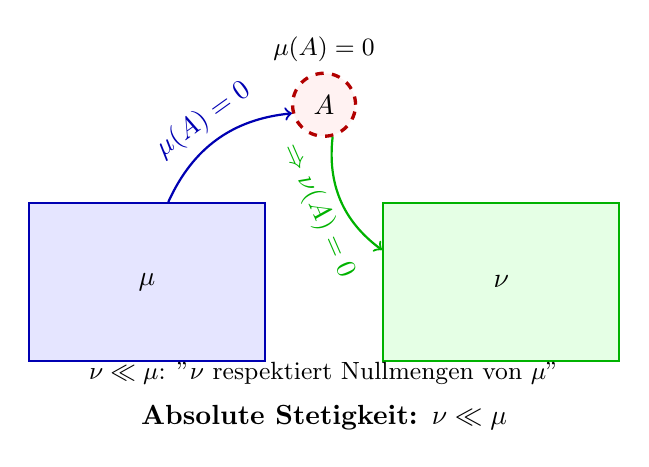
\begin{tikzpicture}[scale=0.9]
    % Referenzmaß mu
    \node[rectangle, draw=blue!70!black, thick, minimum width=3cm, minimum height=2cm, fill=blue!10] (mu) at (0,0) {$\mu$};
    
    % Absolut stetiges Maß nu
    \node[rectangle, draw=green!70!black, thick, minimum width=3cm, minimum height=2cm, fill=green!10] (nu) at (5,0) {$\nu$};
    
    % Nullmenge A
    \node[circle, draw=red!70!black, dashed, very thick, minimum size=0.8cm, fill=red!5] (A) at (2.5, 2.5) {$A$};
    \node[above] at (A.north) {\small $\mu(A) = 0$};
    
    % Pfeile zeigen Implikation
    \draw[->, thick, blue!70!black] (mu) to[bend left=30] node[above, sloped] {$\mu(A) = 0$} (A);
    \draw[->, thick, green!70!black] (A) to[bend right=30] node[below, sloped] {$\Rightarrow \nu(A) = 0$} (nu);
    
    % Symbol
    \node[below] at (2.5, -1) {\small $\nu \ll \mu$: "$\nu$ respektiert Nullmengen von $\mu$"};
    
    % Label
    \node[below] at (2.5, -1.6) {\textbf{Absolute Stetigkeit: $\nu \ll \mu$}};
\end{tikzpicture}
\end{center}
\end{denoobification}

\begin{denoobification}[Radon-Nikodym Theorem]
\textbf{Was besagt das Radon-Nikodym Theorem?}

Wenn $\nu \ll \mu$ und $\mu$ ist $\sigma$-endlich, dann existiert eine (fast überall eindeutige) messbare Funktion $f \geq 0$ mit:
\[
\nu(A) = \int_A f \, d\mu \quad \text{für alle } A \in \mathcal{F}
\]

Die Funktion $f$ heißt \textbf{Radon-Nikodym-Dichte} oder \textbf{Dichte} von $\nu$ bezüglich $\mu$, geschrieben $f = \frac{d\nu}{d\mu}$.

\textbf{Intuition:} Jedes absolut stetige Maß hat eine "Dichte" bezüglich dem Referenzmaß.

\textbf{In der Wahrscheinlichkeit:}
\begin{itemize}
    \item Wahrscheinlichkeitsdichte: $f = \frac{d\mathbb{P}}{d\lambda}$ (bezüglich Lebesgue-Maß)
    \item Bedingte Dichte: $f_{Y|X} = \frac{d\mathbb{P}_{(X,Y)}}{d\mathbb{P}_X}$
\end{itemize}

\textbf{Industrielle Anwendung (Elektrotechnik/Informatik):}
\begin{itemize}
    \item \textbf{Signal-zu-Rausch-Verhältnis (SNR):} Die Dichte $f = \frac{d\mathbb{P}_{\text{Signal}}}{d\mathbb{P}_{\text{Rauschen}}}$ beschreibt das Verhältnis von Signal- zu Rauschleistung - essentiell für Kommunikationssysteme
    \item \textbf{Spektrale Dichte:} Das Leistungsspektrum $S(f) = \frac{dP}{df}$ ist eine Radon-Nikodym-Dichte - beschreibt die Leistungsverteilung über Frequenzen
    \item \textbf{Adaptive Filter:} Bei adaptiven Filtern wird die Dichte $f = \frac{d\mathbb{P}_{\text{Ausgang}}}{d\mathbb{P}_{\text{Eingang}}}$ verwendet, um den Filter anzupassen
    \item \textbf{Fehlerrate-Schätzung:} Die Fehlerrate kann als Dichte $f = \frac{d\mathbb{P}_{\text{Fehler}}}{d\mathbb{P}_{\text{Übertragung}}}$ beschrieben werden
    \item \textbf{Kanal-Charakterisierung:} In der Kommunikationstechnik beschreibt die Radon-Nikodym-Dichte die Kanal-Übertragungsfunktion relativ zu einem Referenzsignal
    \item \textbf{Störungsanalyse:} Die Dichte beschreibt, wie sich Störungen relativ zum ursprünglichen Signal verhalten
\end{itemize}

\textbf{Mars-Kolonisierung Anwendung:}
\begin{itemize}
    \item \textbf{Erd-Mars-Kommunikation SNR:} Die Dichte $f = \frac{d\mathbb{P}_{\text{Signal}}}{d\mathbb{P}_{\text{Rauschen}}}$ beschreibt das Signal-zu-Rausch-Verhältnis über die 225 Millionen km Entfernung - kritisch für Datenübertragung
    \item \textbf{Ressourcen-Dichte:} Die Dichte $f = \frac{d\mathbb{P}_{\text{Ressource}}}{d\mathbb{P}_{\text{Gelände}}}$ beschreibt die Ressourcenverteilung relativ zum Gelände - wichtig für Erkundungsplanung
    \item \textbf{Überlebensrate-Dichte:} Die Dichte $f = \frac{d\mathbb{P}_{\text{Überleben}}}{d\mathbb{P}_{\text{Zeit}}}$ beschreibt die Überlebensrate relativ zur Zeit - wichtig für Langzeitplanung
    \item \textbf{Energie-Effizienz:} Die Dichte $f = \frac{d\mathbb{P}_{\text{Energie-Output}}}{d\mathbb{P}_{\text{Energie-Input}}}$ beschreibt die Energieeffizienz verschiedener Systeme - kritisch für Solarenergie-Management
    \item \textbf{System-Ausfallrate:} Die Dichte $f = \frac{d\mathbb{P}_{\text{Ausfall}}}{d\mathbb{P}_{\text{Betriebszeit}}}$ beschreibt die Ausfallrate relativ zur Betriebszeit - wichtig für Wartungsplanung
    \item \textbf{Produktionsrate:} Die Dichte $f = \frac{d\mathbb{P}_{\text{Produktion}}}{d\mathbb{P}_{\text{Ressourcen}}}$ beschreibt die Produktionsrate (z.B. Sauerstoff, Wasser) relativ zu verfügbaren Ressourcen - essentiell für Selbstversorgung
\end{itemize}

\textbf{Warum wichtig?} Fundamentales Theorem für bedingte Erwartungen und Dichten!

\textbf{$\star$ Mental Model zum Auswendiglernen:}
\begin{itemize}
    \item \textbf{Analogie:} Radon-Nikodym = "Dichte finden" - wenn ein Maß absolut stetig ist, hat es eine Dichte
    \item \textbf{Merksatz:} "$\nu \ll \mu$ → $\nu$ hat Dichte $f$ mit $\nu(A) = \int_A f d\mu$"
    \item \textbf{Visualisierung:} Wie ein "Verhältnis" - die Dichte $f = \frac{d\nu}{d\mu}$ beschreibt, wie $\nu$ relativ zu $\mu$ ist
    \item \textbf{Beispiel:} Wahrscheinlichkeitsdichte = $\frac{d\mathbb{P}}{d\lambda}$ (bezüglich Lebesgue-Maß)
\end{itemize}

\begin{center}
\begin{tikzpicture}[scale=0.9]
    % Referenzmaß mu
    \node[rectangle, draw=blue!70!black, thick, minimum width=3cm, minimum height=2cm, fill=blue!10] (mu) at (0,0) {Referenzmaß $\mu$};
    
    % Absolut stetiges Maß nu
    \node[rectangle, draw=green!70!black, thick, minimum width=3cm, minimum height=2cm, fill=green!10] (nu) at (5,0) {Maß $\nu \ll \mu$};
    
    % Dichte f
    \node[ellipse, draw=red!70!black, thick, minimum width=2cm, minimum height=1cm, fill=red!10] (f) at (2.5,2.5) {Dichte $f$};
    
    % Pfeile
    \draw[->, thick, blue!70!black] (mu) to[bend left=30] node[above, sloped] {$\mu(A) = 0$} (nu);
    \draw[->, thick, green!70!black] (nu) to[bend right=30] node[below, sloped] {$\nu(A) = 0$} (mu);
    \draw[->, thick, red!70!black] (f) to node[right] {$f = \frac{d\nu}{d\mu}$} (nu);
    \draw[->, thick, red!70!black] (f) to node[left] {$\nu(A) = \int_A f d\mu$} (mu);
    
    % Formel
    \node[below] at (2.5, -1) {\small $\nu(A) = \int_A f(\omega) \, d\mu(\omega)$};
\end{tikzpicture}
\end{center}
\end{denoobification}

\section{Multiple-Choice Fragen zur Maßtheorie}

\begin{multiplechoice}
\textbf{Frage 1:} Was ist eine $\sigma$-Algebra?

\begin{enumerate}[label=(\alph*)]
    \item Eine Sammlung von Zahlen
    \item Eine Sammlung von Teilmengen, die abgeschlossen unter Komplementen und abzählbaren Vereinigungen ist
    \item Eine Funktion, die Maße berechnet
    \item Eine Art von Integral
\end{enumerate}

\begin{solution}
\textbf{Richtige Antwort: (b)}

Eine $\sigma$-Algebra $\mathcal{F}$ auf $\Omega$ ist eine Sammlung von Teilmengen von $\Omega$, die:
\begin{itemize}
    \item $\Omega$ enthält
    \item Abgeschlossen unter Komplementen ist
    \item Abgeschlossen unter abzählbaren Vereinigungen ist
\end{itemize}

Sie beschreibt die "messbaren Ereignisse" in einem Wahrscheinlichkeitsraum.
\end{solution}
\end{multiplechoice}

\begin{multiplechoice}
\textbf{Frage 2:} Was bedeutet $\sigma$-Additivität für ein Maß $\mu$?

\begin{enumerate}[label=(\alph*)]
    \item $\mu(A \cup B) = \mu(A) + \mu(B)$ für alle $A, B$
    \item $\mu\left(\bigcup_{i=1}^{\infty} A_i\right) = \sum_{i=1}^{\infty} \mu(A_i)$ für disjunkte Mengen $A_i$
    \item $\mu(A) \geq 0$ für alle $A$
    \item $\mu(\emptyset) = 0$
\end{enumerate}

\begin{solution}
\textbf{Richtige Antwort: (b)}

$\sigma$-Additivität bedeutet, dass für paarweise disjunkte Mengen $A_1, A_2, \ldots$ gilt:
\[
\mu\left(\bigcup_{i=1}^{\infty} A_i\right) = \sum_{i=1}^{\infty} \mu(A_i)
\]

Dies ist eine der fundamentalen Eigenschaften eines Maßes und erlaubt es, mit unendlichen Vereinigungen zu arbeiten.
\end{solution}
\end{multiplechoice}

\begin{multiplechoice}
\textbf{Frage 3:} Wann ist eine Funktion $f: \Omega \to \mathbb{R}$ messbar?

\begin{enumerate}[label=(\alph*)]
    \item Wenn $f$ stetig ist
    \item Wenn $f^{-1}(B) \in \mathcal{F}$ für alle Borel-Mengen $B$
    \item Wenn $f$ beschränkt ist
    \item Wenn $f$ differenzierbar ist
\end{enumerate}

\begin{solution}
\textbf{Richtige Antwort: (b)}

Eine Funktion $f$ ist messbar, wenn für jede Borel-Menge $B \in \mathcal{B}(\mathbb{R})$ das Urbild $f^{-1}(B) = \{\omega : f(\omega) \in B\}$ in $\mathcal{F}$ liegt.

Dies ist äquivalent zu: $f^{-1}((-\infty, a]) \in \mathcal{F}$ für alle $a \in \mathbb{R}$.

Hinweis: Stetige Funktionen sind messbar, aber nicht alle messbaren Funktionen sind stetig!
\end{solution}
\end{multiplechoice}

\begin{multiplechoice}
\textbf{Frage 4:} Was besagt der Satz von Fubini?

\begin{enumerate}[label=(\alph*)]
    \item Integrale können immer vertauscht werden
    \item Integrale über Produkträume können als iterierte Integrale berechnet werden
    \item Alle Funktionen sind integrierbar
    \item Maße sind immer $\sigma$-endlich
\end{enumerate}

\begin{solution}
\textbf{Richtige Antwort: (b)}

Der Satz von Fubini besagt, dass unter geeigneten Bedingungen:
\[
\int_{\Omega_1 \times \Omega_2} f \, d(\mu_1 \otimes \mu_2) = \int_{\Omega_1} \left(\int_{\Omega_2} f \, d\mu_2\right) d\mu_1
\]

Dies erlaubt es, mehrdimensionale Integrale als iterierte eindimensionale Integrale zu berechnen.
\end{solution}
\end{multiplechoice}

\begin{multiplechoice}
\textbf{Frage 5:} Wie erhält man die Randdichte $f_X(x)$ aus der gemeinsamen Dichte $f_{X,Y}(x,y)$?

\begin{enumerate}[label=(\alph*)]
    \item $f_X(x) = f_{X,Y}(x,y)$
    \item $f_X(x) = \int_{-\infty}^{\infty} f_{X,Y}(x,y) \, dy$
    \item $f_X(x) = \int_{-\infty}^{\infty} f_{X,Y}(x,y) \, dx$
    \item $f_X(x) = \frac{f_{X,Y}(x,y)}{f_Y(y)}$
\end{enumerate}

\begin{solution}
\textbf{Richtige Antwort: (b)}

Die Randdichte von $X$ erhält man durch Integration über alle möglichen Werte von $Y$:
\[
f_X(x) = \int_{-\infty}^{\infty} f_{X,Y}(x,y) \, dy
\]

Dies "projiziert" die gemeinsame Dichte auf die $x$-Achse - man "summiert" (integriert) über alle $y$-Werte.

\textbf{Intuition:} Man "vergisst" die Information über $Y$ und betrachtet nur die Verteilung von $X$ allein.
\end{solution}
\end{multiplechoice}

\begin{multiplechoice}
\textbf{Frage 6:} Was besagt das Radon-Nikodym Theorem?

\begin{enumerate}[label=(\alph*)]
    \item Jedes Maß hat eine Dichte
    \item Wenn $\nu \ll \mu$, dann existiert eine Dichte $f$ mit $\nu(A) = \int_A f \, d\mu$
    \item Alle Maße sind absolut stetig
    \item Dichten sind immer eindeutig
\end{enumerate}

\begin{solution}
\textbf{Richtige Antwort: (b)}

Das Radon-Nikodym Theorem besagt: Wenn $\nu \ll \mu$ (absolut stetig) und $\mu$ ist $\sigma$-endlich, dann existiert eine (fast überall eindeutige) messbare Funktion $f \geq 0$ mit:
\[
\nu(A) = \int_A f \, d\mu \quad \text{für alle } A \in \mathcal{F}
\]

Die Funktion $f = \frac{d\nu}{d\mu}$ heißt Radon-Nikodym-Dichte.

\textbf{Wichtig:} Nicht jedes Maß hat eine Dichte - nur absolut stetige Maße!
\end{solution}
\end{multiplechoice}

\section{Zusammenfassung}

Die Maßtheorie liefert das fundamentale mathematische Gerüst für:
\begin{itemize}
    \item \textbf{Wahrscheinlichkeitsräume:} $(\Omega, \mathcal{F}, \mathbb{P})$
    \item \textbf{Zufallsvariablen:} Messbare Funktionen
    \item \textbf{Erwartungswerte:} Lebesgue-Integrale
    \item \textbf{Bedingte Erwartungen:} Radon-Nikodym-Dichten
    \item \textbf{Stochastische Prozesse:} Familien von messbaren Funktionen
\end{itemize}

Ohne diese Grundlagen ist ein tiefes Verständnis der Stochastischen Calculus nicht möglich. Die Konzepte aus diesem Kapitel werden in allen folgenden Kapiteln verwendet.

\textbf{Empfehlung:} Wenn Sie mit diesen Konzepten noch nicht vertraut sind, wiederholen Sie dieses Kapitel, bevor Sie mit Martingalen fortfahren.
